\documentclass[11pt]{article}

\usepackage[T1]{fontenc}
\usepackage{lmodern}
\usepackage[margin=1in]{geometry}
\usepackage{amsmath,amssymb,amsthm}
\usepackage{graphicx}
\usepackage[dvipsnames,table]{xcolor}
\usepackage[round,authoryear]{natbib}
\usepackage{hyperref}
\usepackage{booktabs}
\usepackage{array}
\usepackage{placeins}

\hypersetup{colorlinks=true,linkcolor=MidnightBlue,citecolor=MidnightBlue,urlcolor=NavyBlue}

\graphicspath{{figures/}}

\newtheorem{theorem}{Theorem}
\newtheorem{proposition}{Proposition}
\newtheorem{corollary}{Corollary}
\newtheorem{lemma}{Lemma}
\theoremstyle{remark}
\newtheorem{remark}{Remark}

% Notation shared by all sections. See the conventions table in section 2.
\newcommand{\vth}{v_{\mathrm{th}}}
\newcommand{\gradpar}{\nabla_\parallel}
\newcommand{\kperp}{k_\perp}
\newcommand{\zpm}{z^{\pm}}
\newcommand{\zhat}{\hat{\boldsymbol z}}
\newcommand{\bhat}{\hat{\boldsymbol b}}
\newcommand{\uE}{\boldsymbol u_E}
\newcommand{\dd}{\mathrm{d}}
\newcommand{\ii}{\mathrm{i}}
\newcommand{\Tr}{\mathcal T}
\newcommand{\fe}[2]{[#1,#2]}
\newcommand{\ip}[2]{\langle #1,#2\rangle}
\newcommand{\PVint}{\mathrm{P}\!\!\int}
\newcommand{\Lam}{\Lambda}
\newcommand{\Qphi}{Q_\varphi}
\newcommand{\Hph}{\mathcal H}
\newcommand{\Wc}{W}
\newcommand{\eps}{\varepsilon}
\newcommand{\diel}{\mathcal K}       % dielectric function of a branch
\newcommand{\Pw}{\mathsf P}
% Placeholders for work not yet done (red in the PDF).
\newcommand{\placeholder}[1]{\textcolor{BrickRed}{[\emph{To do:} #1]}}
\newcommand{\placeholderfig}[1]{\fbox{\parbox[c][4.5cm][c]{0.92\textwidth}{\centering\textcolor{BrickRed}{\emph{Figure to come:} #1}}}}


\title{The compressive sector of kinetic reduced magnetohydrodynamics\\ as a continuum of passive scalars}
\author{A. Kanekar}
\date{Draft, \today}

\begin{document}
\maketitle

\begin{abstract}
We show that in kinetic reduced magnetohydrodynamics (KRMHD) the compressive fluctuations are exactly a continuum of passive scalars, or slices, labelled by the parallel phase velocity $u$. The slices are the projections of the compressive distribution on the Case--Van Kampen modes of a velocity-space operator that contains the Landau coupling, is self-adjoint in the free-energy inner product and does not depend on the wavenumber. Without collisions they evolve independently in any smooth three-dimensional Alfv\'enic fields, each carried by the $\boldsymbol E\times\boldsymbol B$ flow and streaming along the perturbed magnetic field at its own speed. The energy of every slice is therefore conserved, which gives an infinite family of quadratic invariants: the free energy and the invariants $\Gamma$ and $\Hph$ of Chandran, Mallet \& Meyrand (2026) weight the slice energies by $1$, $u$ and $1/u$, and $\Gamma$ is the net flux of free energy along the guide field. Phase mixing is the decorrelation of slices by their relative streaming along the field. Fully decorrelated slices give the $m^{-1/2}$ Hermite spectrum of forced linear phase mixing, and since the invariants fix the free energy at each phase velocity but not the correlations between slices, none of them places a Fj{\o}rtoft-type constraint on the transfer of free energy to large Hermite order $m$. A Hermite hierarchy truncated at order $M$ is exactly $M+1$ passive slices for either closure, $g_{M+1}=0$ or $g_{M+1}=g_{M-1}$. For $g_{M+1}=0$ they sit at the Gauss nodes of the Case--Van Kampen spectral measure, and the phase-space helicity of the retained moments is conserved at odd $M$ but not at even $M$. The fastest slice, whose phase velocity grows as $(2M)^{1/2}$, sets the time step of an explicit scheme. We check these results with the GANDALF code.

\end{abstract}

\section{Introduction}\label{sec:intro}

Kinetic reduced magnetohydrodynamics (KRMHD), the limit $k_\perp\rho_i\to0$ of gyrokinetics derived by \citet{Schekochihin2009}, hereafter S09, describes anisotropic fluctuations at scales much larger than the ion gyroradius $\rho_i$ in a strongly magnetised, weakly collisional plasma. Its Alfv\'enic fluctuations obey reduced magnetohydrodynamics and advect the compressive fluctuations, the slow waves and the entropy mode, which obey a kinetic equation for the ion distribution in the parallel velocity $v_\parallel$ and do not act back on them. Without collisions the compressive fluctuations are damped \citetext{\citealp{Barnes1966}; S09} by phase mixing, which transfers their free energy to ever finer structure in $v_\parallel$; this transfer is central to turbulent heating \citep[S09;][]{Schekochihin2016,Meyrand2019,Zhou2023,Adkins2025}. In a Hermite expansion in $v_\parallel$, phase mixing is a flux of free energy to large Hermite order $m$ \citep{Kanekar2015,Schekochihin2016,AdkinsSchekochihin2018,Meyrand2019,Kawazura2020}, and linear phase mixing driven at low $m$ gives a spectrum proportional to $m^{-1/2}$ \citep{ZoccoSchekochihin2011,Kanekar2015}. In KRMHD turbulence \citet{Meyrand2019} found a return flux that cancels much of the phase-mixing flux on average and attributed it to stochastic plasma echoes, in which nonlinear advection returns free energy to low $m$ \citep{KanekarThesis2015,Schekochihin2016,Parker2016,AdkinsSchekochihin2018}.

\citet{Chandran2026}, hereafter CMM, showed that gyrokinetics conserves a second three-dimensional quadratic invariant, the gyrokinetic helicity, and derived its form in KRMHD, where the compressive sector splits into two kinetic branches $G^\pm$ and the Laguerre components of order $l\ge2$ in $v_\perp$ (S09, \S6.2; CMM, appendix~B). In each branch the parallel electric field and the mirror force couple the distribution to its zeroth velocity moment through a term of strength $1/\Lambda^\pm$, which depends only on $\beta_i$ and $T_i/(ZT_e)$; we call this term the Landau coupling. Each branch conserves its free energy $W^\pm$ (S09) and, as CMM found, the phase-space part $\Hph^\pm$ of the helicity and a further quadratic invariant $\Gamma^\pm$. CMM asked whether helicity conservation leads to a bottleneck in velocity space.

We show that the compressive sector of KRMHD is exactly a continuum of independent passive scalars labelled by phase velocity. Because the field relations of KRMHD are algebraic, the branch operator, which combines streaming with the Landau coupling, contains no wavenumber. It is self-adjoint in the free-energy inner product, and its Case--Van Kampen transform \citep{vanKampen1955,Case1959} acts on velocity alone, so it commutes with both nonlinear terms. The slice $a_u$, the transform at $u=v_\parallel/\vth$ with $\vth$ the ion thermal speed, obeys
\begin{equation*}
  \partial_ta_u+\big(\uE+u\vth\,\bhat\big)\cdot\nabla a_u=0,
\end{equation*}
where $\uE$ is the $\boldsymbol E\times\boldsymbol B$ velocity and $\bhat$ the unit vector along the perturbed field. Slices with different $u$ do not interact, in three dimensions and for any smooth Alfv\'enic fields; only velocity-dependent collisions couple them (section~\ref{sec:slices}). The energy of every slice is conserved. The free energy and CMM's $\Gamma$ and $\Hph$ are the integrals of the slice energies over $u$ weighted by $1$, $u$ and $1/u$, any other weight gives a further invariant, and $\Gamma$ is the net free-energy flux along the guide field (section~\ref{sec:invariants}). Phase mixing is the decorrelation of slices by their relative streaming along the field, and slices decorrelated in velocity give the $m^{-1/2}$ spectrum of forced linear phase mixing. Linear phase mixing conserves every invariant of the compressive distribution while it moves all of the free energy to arbitrarily large $m$, so neither the helicity nor any other invariant imposes a constraint of the kind \citet{Fjortoft1953} found for two-dimensional flows, as CMM expected for $\Gamma$ (section~\ref{sec:decorrelation}); this concerns transient solutions, not the forced steady states in which CMM posed their question. A Hermite hierarchy truncated at order $M$, as evolved by Fourier--Hermite codes, consists of exactly $M+1$ slices, which for the closure $g_{M+1}=0$ sit at the Gauss nodes of the Case--Van Kampen spectral measure; the fastest slice sets the time step of an explicit scheme, and the phase-space helicity of the retained moments is conserved only at odd $M$ (section~\ref{sec:truncated}). Section~\ref{sec:numerics} checks these results with the GANDALF code \citep{Kanekar2025}.

Parts of this structure are known elsewhere. The transform is, up to a weight, the inverse of the G-transform of \citet{MorrisonPfirsch1992} and \citet{Morrison1994}, which \citet{Morrison2000} showed to be invertible under the stability condition of \citet{Penrose1960}, and which \citet{SkiffHowes2024} use to infer the electric field over a region from the velocity distribution measured at one point. \citet{Heninger2018} applied it to electrostatic drift kinetics with Boltzmann electrons, where the transformed components have the structure of our slices but remain coupled through the potential (their eq.~85); the energy of each component is conserved there too, although they do not state this. Invariants at each velocity were noted for a linear problem by \citet{PlunkParker2014} and proved for a quasi-two-dimensional nonlinear model by \citet{Plunk2015}, and \citet[\S5.1]{Kunz2015} remarked that the free energy of their pressure-anisotropic generalisation of KRMHD is one of infinitely many invariants, without specifying the others. For the Laguerre components with $l\ge2$, which have no Landau coupling, S09's eqs~(210) and~(212) already make the distribution at each $v_\parallel$ a passively mixed field. The normal fields of truncated drift-fluid and gyrofluid hierarchies \citep{Tassi2015,Tassi2017,Tassi2019,Tassi2023} sit at the zeros of a Hermite polynomial \citep{Tassi2022} and, except one field at $v_\parallel=0$ for an odd number of moments, remain coupled in three dimensions; \citet{ParkerDellar2015} identified the eigenvectors of the truncated Hermite system of linearised Vlasov--Poisson with discrete Case--Van Kampen modes, and \citet{Mandell2024} include the largest Gauss--Hermite node in the time step of the GX code. CMM showed that in gyrokinetics the distribution at $v_\parallel=0$ is advected by the gyroaveraged potential alone. S09 (\S6.3) showed that the kinetic equation is linear in the Lagrangian frame of the $\boldsymbol E\times\boldsymbol B$ flow, and \citet{Kunz2015} restated this for pressure-anisotropic plasmas. \citet{KanekarThesis2015} and the GANDALF paper \citep{Kanekar2025} describe the compressive distribution of KRMHD as a kinetic passive scalar, and \citet{Kanekar2014APS} studied a model kinetic passive scalar advected by a stochastic flow; none of these works decomposes the distribution into slices. Remark~\ref{sl:remlit} in section~\ref{sec:slices} gives further precedents, including two-dimensional ones. What is new here is the exact decomposition of the three-dimensional KRMHD compressive sector into passive slices streaming along the perturbed field lines, in the continuum and in truncated hierarchies, and its consequences.

A companion paper \citep{KanekarPrep} studies the Hermite spectrum of forced KRMHD turbulence. It rests on the frozen-line theorem, by which, when the induction equation is ideal, the volume-integrated single-point statistics of the compressive distribution evolve as in linear phase mixing along the initial field lines. That theorem is proved there without the slices; section~\ref{sec:discussion} gives its slice form.

\section{The compressive sector of KRMHD}\label{sec:model}

For a plasma with one ion species and isothermal electrons, KRMHD \citep{Schekochihin2009} consists of reduced magnetohydrodynamics (RMHD) for the Alfv\'enic fluctuations and a kinetic equation for the compressive ones. We use the form of CMM \citep{Chandran2026}, whose section~3.2 and appendix~B restate and extend S09; their equation numbers refer to arXiv:2607.27981v1. Appendix~\ref{app:notation} compares our notation with that of CMM, S09 and the GANDALF code \citep{Kanekar2025}.

\subsection{Alfv\'enic fields}\label{mod:alfven}

We set the Alfv\'en speed $v_A=1$ unless stated otherwise and take the mean field $\boldsymbol B_0$ along $\zhat$. The stream function $\Phi$ and the flux function $\Psi$ give the $\boldsymbol E\times\boldsymbol B$ velocity $\uE=\zhat\times\nabla_\perp\Phi$ and the perpendicular magnetic fluctuation $\boldsymbol b_\perp\equiv\delta\boldsymbol B_\perp/(4\pi n_im_i)^{1/2}=\zhat\times\nabla_\perp\Psi$, and to first order the unit vector along the field is $\bhat=\zhat+\boldsymbol b_\perp$; both $\uE$ and $\bhat$ are divergence-free. With the bracket $\{f,h\}=\partial_xf\,\partial_yh-\partial_yf\,\partial_xh=\zhat\cdot(\nabla f\times\nabla h)$, advection by $\uE$ is $\{\Phi,\cdot\}$ and the derivative along the field is $\gradpar\equiv\bhat\cdot\nabla=\partial_z+\{\Psi,\cdot\}$. The RMHD equations are \citep[eqs~17--18]{Schekochihin2009}
\begin{equation}\label{eq:rmhd}
  \partial_t\Psi+\{\Phi,\Psi\}=\partial_z\Phi,\qquad
  \partial_t\nabla_\perp^2\Phi+\{\Phi,\nabla_\perp^2\Phi\}=\gradpar\nabla_\perp^2\Psi .
\end{equation}
The first, the induction equation $\partial_t\Psi=\gradpar\Phi$, states that the electric field along the total magnetic field vanishes. Equations (\ref{eq:rmhd}) are CMM's eqs~(3.23)--(3.24) in their normalised potentials (3.2) and do not contain the compressive fluctuations. The Elsasser potentials $z^\pm=\Phi\pm\Psi$ (S09's $\zeta^\pm$) obey $\partial_tz^\pm=\pm\partial_zz^\pm$ linearly, so $z^+$ propagates toward $-z$ and $z^-$ toward $+z$.\footnote{S09's \S\S2.3 and~2.5 write the solutions with $\zeta^\mp=0$ as $\zeta^\pm=f^\pm(x,y,z\mp v_At)$, the opposite direction. We checked ours against S09's eq.~(21), CMM's equations and GANDALF's right-hand side.}

\subsection{Kinetic equation and the two branches}\label{mod:branches}

The ion thermal speed is $\vth=(2T_i/m_i)^{1/2}$, so $s\equiv\vth/v_A=\beta_i^{1/2}$; we write $\tau=T_i/T_e$ and $Z=q_i/e$. The compressive part of the ion distribution is the function $g$ of S09 (CMM's $g_{09}$, their eq.~3.26), which obeys CMM's eq.~(3.25) (S09 eq.~157 without collisions),
\begin{equation}\label{mod:kinetic}
  \frac{\dd g}{\dd t}+v_\parallel\gradpar\Big[g+\Big(\frac{Z}{\tau}\frac{\delta n}{n}+\frac{v_\perp^2}{\vth^2}\frac{\delta B}{B}\Big)F_0\Big]=0,
  \qquad \frac{\dd}{\dd t}=\partial_t+\{\Phi,\cdot\},
\end{equation}
where $F_0$ is the three-dimensional Maxwellian. Quasineutrality and perpendicular pressure balance give (CMM eqs~3.27--3.28; S09 eqs~158--159),
\begin{equation}\label{mod:fields}
  \overline{g}=\frac{\delta n}{n}-\frac{\delta B}{B},\qquad
  \overline{(v_\perp^2/\vth^2)\,g}=-\frac{Z}{\tau}\frac{\delta n}{n}-2\Big(1+\frac{1}{\beta_i}\Big)\frac{\delta B}{B},
  \qquad \overline{(\cdots)}\equiv\frac{1}{n_i}\int\dd^3v\,(\cdots).
\end{equation}
These relations are algebraic: $\delta n/n$ and $\delta B/B$ at a point are linear functionals of $g$ at that point, with coefficients that do not depend on the wavenumber. At finite $k_\perp\rho_i$ they contain gyroaveraging operators.

We expand $g$ in Laguerre polynomials of $v_\perp^2/\vth^2$ with coefficients $G_l(v_\parallel)$ (S09 eq.~205; CMM eq.~B8; appendix~\ref{app:branches}). The source term in (\ref{mod:kinetic}) is linear in $v_\perp^2$, so the coefficients with $l\ge2$ obey $\dd G_l/\dd t+v_\parallel\gradpar G_l=0$ (CMM eq.~B10; S09 eqs~210 and~212). The coefficients with $l=0,1$ are coupled through $\delta n/n$ and $\delta B/B$; the combinations $G^\pm$ of CMM's eqs~(B5)--(B6) (S09 eqs~183--184) obey CMM's eq.~(B4) (S09 eq.~181),
\begin{equation}\label{mod:Gpm}
  \frac{\dd G^\pm}{\dd t}+v_\parallel\gradpar G^\pm
  =\frac{v_\parallel F_M(v_\parallel)}{\Lambda^\pm}\,\gradpar\int G^\pm(v_\parallel')\,\dd v_\parallel',
\end{equation}
where $F_M(v_\parallel)=\pi^{-1/2}\vth^{-1}e^{-v_\parallel^2/\vth^2}$ and
\begin{equation}\label{eq:Lambdapm}
  \Lambda^\pm=-\frac{\tau}{Z}+\frac{1}{\beta_i}\pm\Delta,\qquad
  \Delta=\Big[\Big(1+\frac{\tau}{Z}\Big)^2+\frac{1}{\beta_i^2}\Big]^{1/2}
\end{equation}
(CMM eq.~B7; S09 eqs~182 and~204).\footnote{CMM's eq.~(B16) prints the square root in (\ref{eq:Lambdapm}) as $[(1+\tau/Z)+\beta_i^{-2}]^{1/2}$, without the square on $1+\tau/Z$; with the square, as in S09's eq.~(204), their decompositions (B15) and (B17) hold, and without it they do not (appendix~\ref{app:branches}).} We call the right-hand side of (\ref{mod:Gpm}), of strength $1/\Lambda^\pm$, the Landau coupling; in linear theory it produces the collisionless damping of the compressive fluctuations (S09, \S6.2.2). The coefficients with $l\ge2$ obey (\ref{mod:Gpm}) with $1/\Lambda=0$, and we call them the sector $\Lambda=\infty$. The compressive sector therefore consists of independent kinetic equations for $G^+$, $G^-$ and each $G_l$ with $l\ge2$, all advected by the same Alfv\'enic fields. Since $\Delta>1+\tau/Z$ and $\Delta>1/\beta_i$, $\Lambda^+-1>\beta_i^{-1}$ and $\Lambda^-<-\tau/Z$, so $\Lambda^+>1$ and $\Lambda^-<0$ for all $\beta_i,\tau/Z>0$ (S09, below eq.~200); at $\beta_i=\tau=Z=1$, $\Lambda^\pm=\pm\sqrt5$.

\subsection{One branch in the variable \texorpdfstring{$u$}{u}}\label{mod:onebranch}

We now drop the branch label, set $u=v_\parallel/\vth$, and write $F_M(u)=\pi^{-1/2}e^{-u^2}$ and $M_k[G]=\int u^kG\,\dd u$. Since $v_\parallel=su$ when $v_A=1$, equation (\ref{mod:Gpm}) becomes
\begin{equation}\label{eq:branch}
  \partial_tG+\{\Phi,G\}+s\,\gradpar(LG)=0,
\end{equation}
with the branch operator
\begin{equation}\label{eq:L}
  LG=uG-\frac{uF_M}{\Lambda}\,M_0[G],
\end{equation}
which acts on the velocity variable only; for $\Lambda=\infty$ it is multiplication by $u$. Because the field relations (\ref{mod:fields}) are algebraic, $L$ contains no wavenumber.

For given $\Phi$ and $\Psi$, equation (\ref{eq:branch}) is linear in $G$. Its nonlinear terms are the advection $\{\Phi,G\}$ and the part $s\{\Psi,LG\}$ of the streaming, which follows the perturbed field lines. The Alfv\'enic fields obey (\ref{eq:rmhd}) whatever $G$ does, so the compressive sector is passive. At finite $k_\perp\rho_i$ this fails; the induction equation, for example, contains $\gradpar(\delta n/n)$ (CMM, \S3.1).

The density and field-strength fluctuations are linear combinations of $M_0[G^+]$ and $M_0[G^-]$ (\ref{appA:dndB}), the parallel ion flow involves $M_1[G^\pm]$, and the pressure perturbations involve $M_0[G^\pm]$ and $M_2[G^\pm]$ (appendix~\ref{app:branches}); the sector $\Lambda=\infty$ contributes to none of these moments.

\subsection{Hermite representation}\label{mod:hermite}

Following CMM (eqs~B27 and~B30), we expand $G=\sum_{m\ge0}g_mH_m(u)F_M(u)/\sqrt{2^mm!}$, so that $g_m=\int H_m\,G\,\dd u/\sqrt{2^mm!}$ and $G/F_M^{1/2}=\sum_mg_m\psi_m(u)$ with the orthonormal Hermite functions $\psi_m$. The $g_m$ are CMM's $\tilde G_m$, and $M_0[G]=g_0$, $M_1[G]=g_1/\sqrt2$. In this basis (\ref{eq:branch}) is the hierarchy
\begin{equation}\label{mod:hierarchy}
  \partial_tg+\{\Phi,g\}+s\,\gradpar(Ag)=0,\qquad g=(g_0,g_1,g_2,\dots)^{\mathsf T},
\end{equation}
where the ladder matrix $A$, the matrix of $L$, is tridiagonal with zero diagonal,
\begin{equation}\label{mod:ladder}
  A_{m,m+1}=A_{m+1,m}=\sqrt{\frac{m+1}{2}}\quad\text{except}\quad A_{10}=\frac{1-1/\Lambda}{\sqrt2}.
\end{equation}
The weight matrix $\Pw=\mathrm{diag}(p_m)$, with $p_0=1-1/\Lambda$ and $p_m=1$ for $m\ge1$, symmetrises it, $\Pw A=(\Pw A)^{\mathsf T}$, and $\sum_mp_mg_m^2$ is the free-energy product $\fe{G}{G}$ of section~\ref{sec:slices}. A truncation at $m=M$ needs a closure; by default we use the zero closure $g_{M+1}=0$, which keeps the first $M+1$ rows and columns of $A$. GANDALF \citep{Kanekar2025} integrates (\ref{eq:rmhd}) in Elsasser form together with (\ref{mod:hierarchy}) for one branch, with optional dissipation, hypercollisions and forcing, truncated with the zero closure or with the copy closure $g_{M+1}=g_{M-1}$ (section~\ref{sec:truncated}). We checked to round-off that its right-hand side without dissipation and hypercollisions is (\ref{mod:hierarchy})--(\ref{mod:ladder}), for both signs of $\Lambda$ and both closures.

The rest of the paper concerns one equation (\ref{eq:branch}) with $\Lambda\notin[0,1]$, which we call a branch whether it describes $G^\pm$ or a Laguerre coefficient with $l\ge2$, and treats a collisionless and unforced branch except where stated. The Hermite spectrum of the free energy is $W(m)=p_m\langle g_m^2\rangle$, where $\langle\cdot\rangle$ is the average over the periodic box, so that $\sum_mW(m)=\langle\fe{G}{G}\rangle$.

\section{Phase-velocity slices}\label{sec:slices}

This section shows that each branch (\ref{eq:branch}) is a continuum of passive scalars, or slices, labelled by the parallel phase velocity. The Alfv\'enic fields $\Phi$ and $\Psi$ are given functions of $\boldsymbol r$ and $t$; (\ref{eq:rmhd}) is not used.

\subsection{Without the Landau coupling}\label{sl:nocoupling}

For $\Lambda=\infty$ the operator $L$ is multiplication by $u$, and (\ref{eq:branch}) holds separately at every $u$:
\begin{equation*}
  \partial_tG+\{\Phi,G\}+su\,\gradpar G=0 .
\end{equation*}
Since $\gradpar=\partial_z+\{\Psi,\cdot\}$ and $\{f,G\}=(\zhat\times\nabla_\perp f)\cdot\nabla G$, this is the advection equation $\partial_tG+\boldsymbol U_u\cdot\nabla G=0$ with the velocity
\begin{equation}\label{eq:Uu}
  \boldsymbol U_u=\zhat\times\nabla_\perp(\Phi+su\Psi)+su\,\zhat=\uE+su\,\bhat,\qquad\nabla\cdot\boldsymbol U_u=0 .
\end{equation}
At each $u$, $G$ is a passive scalar, carried by the $\boldsymbol E\times\boldsymbol B$ flow and streaming along the perturbed field at the speed $su$, which is the motion of the guiding centre of a free ion with $v_\parallel=u\vth$. Values of $G$ at different $u$ do not interact. This is the exact equation for the Laguerre coefficients $G_l$ with $l\ge2$ (S09, eqs~210 and~212).

\subsection{With the Landau coupling}\label{sl:transformsec}

For finite $\Lambda$, $LG=uG-(uF_M/\Lambda)\,M_0[G]$ ties every velocity to the density $M_0[G]$, through the parallel electric field and the mirror force, so $G$ at fixed $u$ is no longer a passive scalar. The slices survive in other variables. The reason is that $L$ acts on velocity only and is the same at every point and at every wavenumber, because the field relations (\ref{mod:fields}) are algebraic. A change of velocity variables that diagonalises $L$ therefore does so everywhere at once, and it passes through the advection and the streaming unchanged.

The argument is clearest for the hierarchy (\ref{mod:hierarchy}) truncated at $m=M$ with the zero closure, in which $L$ is the constant $(M+1)\times(M+1)$ matrix $A$. Let $\boldsymbol w_j$ be a left eigenvector of $A$, $\boldsymbol w_j^{\mathsf T}A=u_j\boldsymbol w_j^{\mathsf T}$. Since $\boldsymbol w_j$ does not depend on position or time, it passes through $\partial_t$, $\partial_z$ and both brackets, and multiplying (\ref{mod:hierarchy}) by $\boldsymbol w_j^{\mathsf T}$ gives for $a_j=\boldsymbol w_j^{\mathsf T}g$
\begin{equation*}
  \partial_ta_j+\{\Phi,a_j\}+su_j\,\gradpar a_j
  =\partial_ta_j+\{\Phi+su_j\Psi,\,a_j\}+su_j\,\partial_za_j=0 .
\end{equation*}
Each $a_j$ is a passive scalar, advected with the stream function $\Phi+su_j\Psi$ and streaming along $z$ at the speed $su_j$, as $G$ at fixed $u$ was for $\Lambda=\infty$, and nothing couples $a_j$ to the other $a_l$. The nonlinearity enters only through the bracket with $\Phi+su_j\Psi$, and the Landau coupling does not appear, because it has been absorbed into $\boldsymbol w_j$. For the $a_j$ to be a change of variables, the $u_j$ must be real and the $\boldsymbol w_j$ linearly independent, so that the $a_j$ determine $g$. Both hold because $\Pw A$ is symmetric (section~\ref{mod:hermite}): $A$ is self-adjoint in the free-energy product $\sum_mp_mg_mh_m$, which is positive definite when $p_0=1-1/\Lambda>0$, that is, for $\Lambda\notin[0,1]$. Section~\ref{sec:truncated} normalises the $a_j$ and treats both closures.

At $M=\infty$ the same steps need the eigenfunctions of $L$ itself. Self-adjointness carries over: $L$ is self-adjoint in the free-energy product
\begin{equation}\label{eq:fe}
  \fe{f}{g}=\int\frac{fg}{F_M}\,\dd u-\frac{M_0[f]\,M_0[g]}{\Lambda},
\end{equation}
which is $\sum_mp_mf_mg_m$ in the Hermite variables and is positive definite for $\Lambda\notin[0,1]$, as for every compressive branch of KRMHD ($\Lambda^+>1$, $\Lambda^-<0$; section~\ref{sec:model}). Unlike $A$, however, $L$ has no eigenfunctions of finite free energy: its spectrum is the whole real line and is continuous. Its generalised eigenfunctions are the Case--Van Kampen modes $F_u$ of the branch \citep{vanKampen1955,Case1959}, with $LF_u=uF_u$ for every real $u$. Each is a beam of particles at $v_\parallel=u\vth$, a $\delta$-function in velocity, dressed by the response of the Maxwellian, through the Landau coupling, to the density of the beam (appendix~\ref{app:spectral}). The projection $\Tr[G](u)=\fe{F_u}{G}$ on $F_u$ takes the place of $\boldsymbol w_j^{\mathsf T}g$, and its unit-weight form is the slice amplitude
\begin{equation}\label{eq:aunit}
  a_u=\sqrt{\varrho(u)}\;\fe{F_u}{G},\qquad \varrho(u)=\frac{F_M(u)}{|\diel(u+\ii0)|^2},
\end{equation}
where $\diel$ is the dielectric function of the branch, which contains the plasma dispersion function, and $\varrho$ is the spectral density of the branch, positive with $\int\varrho\,\dd u=1/p_0$. For $\Lambda=\infty$, $F_u$ is the bare beam, $\diel=1$, $\varrho=F_M$ and $a_u=G/\sqrt{F_M}$. The map $G\mapsto a_u$ is a fixed linear change of variables in velocity. It is invertible, divides the free energy among phase velocities without cross terms, and turns $L$ into multiplication by $u$:
\begin{equation}\label{sl:parseval}
  \fe{G}{G}=\int a_u^2\,\dd u,\qquad G\mapsto a_u\ \text{ takes }\ LG\mapsto u\,a_u
\end{equation}
(theorem~\ref{thm:spectrum}, which also gives $a_u$ in terms of $G$ and its Hilbert transform in $u$). Its inverse is, up to normalisation, the G-transform that \citet{MorrisonPfirsch1992} and \citet{Morrison2000} introduced for linearised Vlasov--Poisson; \citet{Heninger2018} applied it to electrostatic drift kinetics, where the transformed components remain coupled through the potential.

\subsection{The slice theorem}\label{sl:slicesec}

\begin{theorem}\label{thm:slice}
Assume that (i) $\Lambda\notin[0,1]$, the value $\Lambda=\infty$ included; (ii) $\Phi(\boldsymbol r,t)$ and $\Psi(\boldsymbol r,t)$ are real functions on $\mathbb T^3\times[0,t_1]$, with $\mathbb T^3$ a periodic box, whose gradients are continuous and Lipschitz in $\boldsymbol r$, uniformly in $t$; they need not satisfy (\ref{eq:rmhd}) and may obey resistive or forced RMHD, or be prescribed; (iii) $G$ and $uG$ are continuously differentiable functions of $(\boldsymbol r,t)$ with values in the space $\mathcal W$ of functions of $u$ with finite $\int G^2F_M^{-1}\,\dd u$ (appendix~\ref{app:spectral}). Then $G$ solves (\ref{eq:branch}) if and only if, at every $(\boldsymbol r,t)$ and for almost every $u$,
\begin{equation}\label{eq:slice}
  \partial_ta_u+\boldsymbol U_u\cdot\nabla a_u=\partial_ta_u+\{\Phi+su\Psi,\,a_u\}+su\,\partial_za_u=0,
\end{equation}
with $\boldsymbol U_u$ of (\ref{eq:Uu}).
\end{theorem}

\begin{proof}
This is the argument for the truncated hierarchy in section~\ref{sl:transformsec}, with the map $\mathcal A:G\mapsto a$ of (\ref{eq:aunit}) in place of $\boldsymbol w_j^{\mathsf T}$. The map $\mathcal A$ is bounded and injective (theorem~\ref{thm:spectrum}) and acts on $u$ only, through a kernel independent of $\boldsymbol r$ and $t$, so it commutes with $\partial_t$, with spatial derivatives and with multiplication by functions of $(\boldsymbol r,t)$, hence with $\{\Phi,\cdot\}$, $\{\Psi,\cdot\}$ and $\gradpar$. With $\mathcal ALG=u\,\mathcal AG$ this gives $\mathcal A[\partial_tG+\{\Phi,G\}+s\,\gradpar(LG)]=\partial_ta+\{\Phi,a\}+su\,\gradpar a$, and $u\,\gradpar a_u=u\,\partial_za_u+\{u\Psi,a_u\}$ gives (\ref{eq:slice}). Since $\mathcal A$ is linear and injective, $G$ solves (\ref{eq:branch}) if and only if $a$ solves (\ref{eq:slice}).
\end{proof}

With the Landau coupling, therefore, each slice is again a passive scalar carried by $\boldsymbol U_u$, in three dimensions, and slices with different $u$ do not interact. The parallel electric field and the mirror force, which enter through the Landau coupling, only dress the slices: the distribution at fixed $u$ is not a passive scalar, but its projection $a_u$ on $F_u$ is. Since $\boldsymbol U_u$ is divergence-free, each slice keeps its own free energy $\int a_u^2\,\dd^3\boldsymbol r$, and by (\ref{sl:parseval}) the nonlinearity moves no free energy between phase velocities (section~\ref{sec:invariants}). In terms of the Elsasser potentials, the stream function of the slice at $u$ is
\begin{equation}\label{eq:elsasserpot}
  \Phi+su\Psi=\tfrac12\big[(1+su)\,z^++(1-su)\,z^-\big],
\end{equation}
so the slices at $su=-1$ and $+1$ are advected by $z^-$ alone and by $z^+$ alone, and the slice at $u=0$ by $\Phi$ alone (section~\ref{sl:special}). The sectors have different transforms, but $\boldsymbol U_u$ depends only on $u$, so at each $u$ the slices of $G^+$, $G^-$ and every $G_l$ with $l\ge2$ are carried by the same flow:
\begin{equation}\label{eq:sameflow}
  \big(\partial_t+\boldsymbol U_u\cdot\nabla\big)\big(a^+_u,\,a^-_u,\,a^{(2)}_u,\,a^{(3)}_u,\dots\big)=0 .
\end{equation}
The compressive sector of KRMHD is therefore a continuum of passive scalars labelled by phase velocity. Section~\ref{sec:truncated} shows that a truncated Hermite hierarchy decomposes in the same way, and figure~\ref{fig:snapshots} (section~\ref{sec:numerics}) shows three slices of a GANDALF run that start from the same density pattern and are carried apart by their own flows.

\subsection{Special slices}\label{sl:special}

The slice $u=0$ is advected by $\uE$ alone. If $G$ is H\"older continuous in $u$ near $u=0$, (\ref{eq:transform}) gives $\Tr[G](0)=p_0\,G(0)/F_M(0)$, so this slice is the distribution at $v_\parallel=0$, which obeys $\partial_tG+\{\Phi,G\}=0$ there because $(LG)(0)=0$. This is the KRMHD form of CMM's eq.~(2.22), by which in gyrokinetics the distribution at $v_\parallel=0$ is advected by the gyroaveraged potential alone. Section~\ref{sec:invariants} relates the energy of this slice to the imaginary part of CMM's complex helicity, and section~\ref{sec:truncated} gives its truncated counterpart.

\begin{proposition}\label{prop:elsasser}
Under the hypotheses of theorem~\ref{thm:slice}, the slices with $su=-1$ and $su=+1$, that is, with $v_\parallel=-v_A$ and $+v_A$, obey
\begin{equation}\label{sl:elsasser}
  (\partial_t-\partial_z)\,a_u+\{z^-,a_u\}=0\quad(su=-1),\qquad
  (\partial_t+\partial_z)\,a_u+\{z^+,a_u\}=0\quad(su=+1).
\end{equation}
The slice $su=-1$ moves toward $-z$ with $z^+$ and is advected by $z^-$ alone, and the slice $su=+1$ moves toward $+z$ with $z^-$ and is advected by $z^+$ alone. In a truncated hierarchy the same holds for a slice of theorem~\ref{thm:trunc} whose speed $su_j$ is $-1$ or $+1$.
\end{proposition}

\begin{proof}
By (\ref{eq:elsasserpot}), $\Phi+su\Psi$ is $z^-$ at $su=-1$ and $z^+$ at $su=+1$. Substituting in (\ref{eq:slice}) gives (\ref{sl:elsasser}).
\end{proof}

The two slices exist at every $\beta_i$, at $u=\pm\beta_i^{-1/2}$ (in a truncated hierarchy only when $\beta_i=u_j^{-2}$ for an eigenvalue $u_j$), whereas the fluid slow waves interact exclusively with the counter-propagating Alfv\'en waves only for $\beta\gg1$ \citetext{S09, \S2.5, eq.~30 and footnote~15; \citealp[\S2.4]{LithwickGoldreich2001}}. The fluid slow waves and the entropy mode of S09 (their eqs~23 and~29--30) obey (\ref{eq:slice}) at $su=\mp c$, with $c$ the slow-wave speed in units of $v_A$, and at $u=0$; this is a formal correspondence, not a derived collisional limit of the slices.

The equations (\ref{eq:rmhd}) and (\ref{eq:branch}) are invariant under the reflection
\begin{equation}\label{eq:mirror}
  \Phi'(\boldsymbol r)=\Phi(\tilde{\boldsymbol r}),\qquad
  \Psi'(\boldsymbol r)=-\Psi(\tilde{\boldsymbol r}),\qquad
  G'(\boldsymbol r,u)=G(\tilde{\boldsymbol r},-u),\qquad
  \tilde{\boldsymbol r}=(x,y,-z),
\end{equation}
which reverses $z$ and $v_\parallel$, exchanges $z^+$ and $z^-$, and maps the slice at $u$ to the slice at $-u$, $a'_u(\boldsymbol r)=a_{-u}(\tilde{\boldsymbol r})$. The free energy $\Wc$ is therefore even under (\ref{eq:mirror}), and $\Gamma$ and $\Hph$, which weight the slice energies with $u$ and $1/u$ (section~\ref{sec:invariants}), are odd, so they vanish in every state that is its own mirror image.

\subsection{Dissipation, collisions and forcing}\label{sl:forcingsec}

Let the right-hand side of (\ref{eq:branch}) be $-\mathcal BG-\mathcal CG+F$, where the linear operators $\mathcal B$ and $\mathcal C$ act on $\boldsymbol r$ alone and on $u$ alone, respectively, and $F$ is a source. The proof of theorem~\ref{thm:slice} gives
\begin{equation}\label{eq:sliceforcing}
  \partial_ta_u+\boldsymbol U_u\cdot\nabla a_u=-\mathcal B\,a_u-\int\hat{\mathcal C}(u,u')\,a_{u'}\,\dd u'+\sqrt{\varrho(u)}\;\Tr[F](u),
\end{equation}
where $\hat{\mathcal C}$ is the kernel of $\mathcal A\,\mathcal C\,\mathcal A^{-1}$. Damping at a rate that depends only on $k_\perp$ or $k_z$, applied with the same coefficient to every Hermite moment, is of the form $\mathcal B$ and damps each slice separately. With $e_m=H_m(u)F_M(u)/\sqrt{2^mm!}$ and $r_m(u)$ the $m$th Hermite coefficient of $F_u$, a polynomial of degree $m$ with $r_0=1$ and $r_1=\sqrt2\,u$, one has $\Tr[e_m](u)=p_m\,r_m(u)$, and the functions $\phi_m=\sqrt{p_m\varrho}\;r_m$ form an orthonormal basis of $L^2(\mathbb R,\dd u)$. For $\mathcal Ce_m=\nu_me_m$, as for Lenard--Bernstein collisions ($\nu_m=\nu m$) or hypercollisions ($\nu_m=\nu(m/M)^n$), the kernel is $\hat{\mathcal C}(u,u')=\sum_m\nu_m\,\phi_m(u)\,\phi_m(u')$, which couples different slices unless all $\nu_m$ are equal; collisions are the only term in (\ref{eq:sliceforcing}) that exchanges free energy between slices. Forcing of $g_0$ by a field $f(\boldsymbol r,t)$, $F=f\,e_0$, gives every slice the same spatial pattern, with amplitude $(1-1/\Lambda)\sqrt{\varrho(u)}\,f$.

\begin{remark}\label{sl:remlit}
Parts of this structure are known in other settings. For $\Lambda=\infty$, theorem~\ref{thm:slice} restates S09's eqs~(210) and~(212), which describe the Laguerre components with $l\ge2$ as a passively mixed, undamped ballistic-type mode; the transform adds the two branches, absorbing their Landau coupling into the slices. \citet[section~IV]{Heninger2018} applied the G-transform to the electrostatic drift-kinetic ion equation with Boltzmann electrons in a slab \citep[see also][chapter~13]{Heninger2020}, where quasineutrality also makes the kernel independent of the wavenumber; their transform is ours with $\Lambda=-T_i/(ZT_e)$, the limit of $\Lambda^-$ as $\beta_i\to0$. Their transformed components stream along the uniform guide field and share one $\boldsymbol E\times\boldsymbol B$ flow but remain coupled through the potential, which is proportional to $\int g\,\dd v_\parallel$; their equation also conserves the energy of each component in three dimensions, although they do not state this. In linear problems at a single wavenumber the transform was used by \citet{Plunk2013}, for a forced Landau problem, and by \citet{PlunkParker2014}, who noted that without forcing any $u$-weighted integral of the squared transformed distribution is conserved, and \citet{Plunk2015} used a transform that commutes with $\boldsymbol E\times\boldsymbol B$ advection to obtain a quadratic invariant at each velocity, and from it the nonlinear stability of a quasi-two-dimensional drift-kinetic model without parallel streaming.

Invariants labelled by a velocity variable are known in two dimensions. In two-field models of collisionless reconnection, two Lagrangian invariants are advected by the generalised stream functions $\phi\pm(\rho_s/d_e)\psi$ \citep{Schep1994,Cafaro1998,Grasso2001}, and in their drift-kinetic version the distribution at each value of the parallel canonical momentum is a Lagrangian invariant \citep{Liseikina2004,Pegoraro2004}. Two-dimensional gyrokinetics has an invariant for every pair $(v_\perp,v_\parallel)$ \citetext{S09, appendix~F.1; \citealp[\S3]{Plunk2010}}, and \citet{ZhuHammett2010} used per-velocity quadratic invariants that survive Galerkin truncation to construct its absolute equilibria; the low-beta equations of \citet{ZoccoSchekochihin2011} have Lagrangian invariants parametrised by $v_\parallel$. In each of these models the terms with parallel gradients break the invariants in three dimensions.
\end{remark}

\section{Invariants}\label{sec:invariants}

This section derives the invariants of one compressive branch from theorem~\ref{thm:slice}, under its hypotheses, the value $\Lam=\infty$ included, with no collisions, dissipation or sources acting on $G$. We write $\langle\cdot\rangle$ for the average over the periodic box, of volume $V$.

\subsection{The quadratic family}\label{inv:family}

For a function $\varphi$ on the real line, $\varphi(L)$ is defined by the functional calculus of the self-adjoint operator $L$ (theorem~\ref{thm:spectrum}), so that the slice amplitude of $\varphi(L)G$ is $\varphi(u)\,a_u$. Because $G\mapsto a$ is unitary from $(\mathcal W,\fe{\cdot}{\cdot})$ onto $L^2(\mathbb R,\dd u)$,
\begin{equation}\label{eq:Qphi}
  \Qphi\equiv\int\dd^3r\,\fe{G}{\varphi(L)G}=\int\dd u\;\varphi(u)\int\dd^3r\,a_u^2=V\!\int\varphi(u)\,\mathcal E(u)\,\dd u,
  \qquad \mathcal E(u)\equiv\langle a_u^2\rangle ,
\end{equation}
where for unbounded $\varphi$ the last two expressions define $\Qphi$ whenever the integral converges. The slice energy $\mathcal E(u)$ is the distribution of free energy over phase velocity: $\tfrac12n_iT_i\,\mathcal E(u)\,\dd u$ is the free energy per unit volume in the slices with phase velocities in $[u,u+\dd u]$.

\begin{proposition}\label{inv:energy}
Under the hypotheses of this section the slice energy $\mathcal E(u)$ is independent of time. Hence $\Qphi$ is constant for every $\varphi$ for which the integral in (\ref{eq:Qphi}) exists at $t=0$, either absolutely or, for $\varphi=1/u$, as a principal value.
\end{proposition}

\begin{proof}
By (\ref{eq:Uu}) and $\nabla\cdot\boldsymbol U_u=0$, $\partial_ta_u^2+\nabla\cdot(\boldsymbol U_u\,a_u^2)=0$, and integration over the periodic box gives $\dd\mathcal E(u)/\dd t=0$.
\end{proof}

For $\varphi(u)=u^n$ the integral converges absolutely when $\int\dd^3r\int(1+u^{2k})\,G^2F_M^{-1}\,\dd u<\infty$ for an integer $k\ge n/2$: $|u|^n\le1+u^{2k}$, and $\int u^{2k}a_u^2\,\dd u=\fe{L^kG}{L^kG}$ is finite when $G$ lies in the domain of $L^k$, which by (\ref{eq:LUP}) is that of $U^k$, because $P-I$ has rank one and its range, spanned by $F_M$, lies in the domain of every power of $U$. For $\varphi(u)=1/u$ the integral is a principal value, which exists when $G(\boldsymbol r,\cdot)$ is H\"older continuous near $u=0$, uniformly in $\boldsymbol r$, because $a_u$, by (\ref{eq:aunit}) a combination of $G$ and its Hilbert transform with coefficients smooth in $u$, is then H\"older continuous there.

Per-velocity quadratic invariants are known in the simpler settings of remark~\ref{sl:remlit} \citep{PlunkParker2014,Plunk2015}, and, unstated, in the transformed equation of \citet[eq.~85]{Heninger2018}. \citet[\S5.1]{Kunz2015} remarked that the free energy of their collisionless pressure-anisotropic generalisation of KRMHD is one of infinitely many invariants, without specifying the others.

\subsection{The invariants \texorpdfstring{$W$, $\Gamma$ and $\Hph$}{W, Gamma and H}}\label{inv:cmm}

The free energy $W^\pm$ of each branch (CMM's B13) is conserved (S09), and CMM found two further quadratic invariants for each branch, the phase-space helicity $\Hph^\pm$ (their B18) and $\Gamma^\pm$ (their B25). Written in $u=v_\parallel/\vth$, with $G^\pm(v_\parallel)\,\dd v_\parallel=G^\pm(u)\,\dd u$, they are the members $\varphi=1$, $u$ and $1/u$ of (\ref{eq:Qphi}):
\begin{equation}\label{eq:WGH}
\begin{aligned}
  W^\pm&=\frac{n_iT_i}{2}\,\big\langle\fe{G^\pm}{G^\pm}\big\rangle=\frac{n_iT_i}{2}\int\mathcal E^\pm(u)\,\dd u,\\
  \Gamma^\pm&=\frac{\vth}{2}\,\big\langle\fe{G^\pm}{LG^\pm}\big\rangle=\frac{\vth}{2}\int u\,\mathcal E^\pm(u)\,\dd u,\\
  \Hph^\pm&=\frac{n_iT_i}{2\vth}\,\Big\langle\PVint\frac{(G^\pm)^2}{uF_M}\,\dd u\Big\rangle=\frac{n_iT_i}{2\vth}\,\PVint\frac{\mathcal E^\pm(u)}{u}\,\dd u ,
\end{aligned}
\end{equation}
where $L$, $\fe{\cdot}{\cdot}$ and $\mathcal E^\pm$ are those of branch $\pm$, $\vth=s$ in units with $v_A=1$, and the second form of $\Hph^\pm$ uses (\ref{inv:pv}) below. The normalisations are CMM's: $W^\pm$ carries the factor $n_iT_i$ and $\Gamma^\pm$ does not, so that $n_iT_i\Gamma^\pm$ has the dimensions of $\vth W^\pm$. CMM's (B14) and (B19) for the Laguerre sectors with $l\ge2$ are the members $\varphi=1$ and $1/u$ at $\Lam=\infty$, summed over $l$. The Hermite forms $\fe{G}{G}=\sum_mp_mg_m^2$ and $\fe{G}{LG}=g^{\mathsf T}\Pw Ag$ give CMM's (B31) and (B32), with the prefactors of (\ref{eq:WGH}); on $M+1$ retained moments with odd $M$, the Hermite matrix of the helicity is the inverse of the ladder matrix at $\Lam=\infty$ (section~\ref{sec:truncated}).

The kernel of $\Hph^\pm$ contains no $\Lam$: by $PL^{-1}=U^{-1}$, which follows from (\ref{eq:LUP}), $\fe{G}{L^{-1}G}=\int G^2(uF_M)^{-1}\,\dd u$ when $G/u$ lies in $\mathcal W$. For a general $G$, the resolvent form $R_G(z)=\fe{G}{(z-L)^{-1}G}$, $\mathrm{Im}\,z>0$, is the Stieltjes transform $\int a_u^2(z-u)^{-1}\,\dd u$ of $a_u^2$ (theorem~\ref{thm:spectrum}), and appendix~\ref{appB:stone} gives $R_G(z)=\int G^2(z-u)^{-1}F_M^{-1}\,\dd u-(z/\Lam)\,C_G(z)^2/\eps(z)$, with $C_G(z)=\int G(v)\,(z-v)^{-1}\,\dd v$. For $G$ H\"older continuous near $u=0$ and $z=\ii\eta$, $\eta\to0^+$, the last term vanishes, because $C_G(\ii\eta)$ stays bounded and $\eps(\ii\eta)\to1-1/\Lam\neq0$, and the Sokhotski--Plemelj formula gives, at every point $\boldsymbol r$,
\begin{equation}\label{inv:pv}
  \PVint\frac{a_u^2}{u}\,\dd u=\PVint\frac{G^2}{uF_M}\,\dd u,\qquad a_0^2=\frac{G(0)^2}{F_M(0)} .
\end{equation}

CMM's gyrokinetic helicity (their 2.15) has the weight $1/(v_\parallel-\ii0)$, and the imaginary part of their Plemelj split (2.17) comes from $v_\parallel=0$. The branch analogue is the member $\varphi(u)=1/(u-\ii0)=\mathrm P(1/u)+\ii\pi\delta(u)$ of the family, and by (\ref{eq:aunit}) and (\ref{inv:pv})
\begin{equation}\label{eq:Hcomplex}
  \Hph^\pm_{\mathrm c}\equiv\frac{n_iT_i}{2\vth}\Big\langle\int\frac{(G^\pm)^2}{(u-\ii0)F_M}\,\dd u\Big\rangle
  =\Hph^\pm+\ii\,\frac{\pi n_iT_i}{2\vth}\,\Big\langle\frac{G^\pm(\boldsymbol r,0,t)^2}{F_M(0)}\Big\rangle .
\end{equation}
The imaginary part, $\pi n_iT_i\,\mathcal E^\pm(0)/(2\vth)$, is proportional to the energy of the slice at $u=0$, which is advected by $\uE$ alone (section~\ref{sec:slices}) and conserved by proposition~\ref{inv:energy}. This is the KRMHD form of CMM's conservation of $\mathrm{Im}\,\Hph$ at each $v_\perp$ (their 2.23).

\subsection{Non-quadratic and cross-sector invariants}\label{inv:casimirs}

Each slice is a Lagrangian invariant of the volume-preserving flow of $\boldsymbol U_u$, so for every $u$ and every function $\mathcal F$ for which the integral exists
\begin{equation}\label{eq:casimir}
  \frac{\dd}{\dd t}\int\dd^3r\,\mathcal F(a_u)=0 .
\end{equation}
By (\ref{eq:sameflow}), the slices $a^\pm_u$ of the two branches and $a^{(l)}_u=G_l(u)/F_M(u)^{1/2}$ of the Laguerre sectors with $l\ge2$ share this flow, so that
\begin{equation}\label{eq:crosssector}
  \frac{\dd}{\dd t}\int\dd^3r\,\mathcal F\big(a^+_u,a^-_u,a^{(2)}_u,a^{(3)}_u,\dots\big)=0,\qquad\text{for example}\qquad\frac{\dd}{\dd t}\int\dd^3r\,a^+_u\,a^-_u=0,
\end{equation}
and integrating the last relation over $u$ with any weight gives quadratic invariants that couple the two branches. Under Fourier--Galerkin truncation in $\boldsymbol r$ only the quadratic members survive (section~\ref{sec:numerics}). Two-dimensional precedents are listed in remark~\ref{sl:remlit}. In three dimensions, \citet{Tassi2022} found in Hermite truncations of drift-kinetic models with an odd number of moments one field that is advected by the $\boldsymbol E\times\boldsymbol B$ flow alone \citep[see also][\S3.4]{Tassi2023} and has an infinite family of Casimirs, the truncated counterpart of the slice at $u=0$; invariants of the form (\ref{eq:casimir}) follow, unstated, from the transformed equation of \citet{Heninger2018}, whose components stream along the uniform guide field. For $u\neq0$, where the slices stream along the perturbed field lines, the non-quadratic members of (\ref{eq:casimir}) and the cross-sector invariants (\ref{eq:crosssector}) that involve the branches $G^\pm$ are new; for the sectors with $l\ge2$ alone they follow, unstated, from S09's eq.~(212).

\subsection{The local conservation law and \texorpdfstring{$\Gamma$}{Gamma} as a flux}\label{inv:flux}

\begin{proposition}\label{prop:localflux}
Under the same hypotheses, the free-energy density per unit $n_iT_i$, $w=\tfrac12\fe{G}{G}$, and the density $\gamma=\tfrac{s}{2}\fe{G}{LG}$ satisfy, at every point,
\begin{equation}\label{eq:localflux}
  \partial_tw+\nabla\cdot\big(w\,\uE+\gamma\,\bhat\big)=0 .
\end{equation}
In slice variables $w=\tfrac12\int a_u^2\,\dd u$ and $\gamma=\tfrac{s}{2}\int u\,a_u^2\,\dd u$, so that $w\,\uE+\gamma\,\bhat=\tfrac12\int a_u^2\,\boldsymbol U_u\,\dd u$.
\end{proposition}

\begin{proof}
The product $\fe{\cdot}{\cdot}$ acts on $u$ at fixed $\boldsymbol r$ with a kernel that does not depend on $\boldsymbol r$, so every derivation $D$ in $\boldsymbol r$ satisfies $D\fe{f}{h}=\fe{Df}{h}+\fe{f}{Dh}$. Both $\{\Phi,\cdot\}$ and $\gradpar$ are such derivations, and both commute with $L$. Since $L$ is symmetric in $\fe{\cdot}{\cdot}$ at each point, $\gradpar\fe{G}{LG}=\fe{\gradpar G}{LG}+\fe{G}{\gradpar LG}=2\,\fe{G}{\gradpar LG}$. Taking $\fe{G}{\cdot}$ of (\ref{eq:branch}) therefore gives $\partial_tw+\{\Phi,w\}+\gradpar\gamma=0$, and $\{\Phi,w\}=\nabla\cdot(w\,\uE)$ and $\gradpar\gamma=\nabla\cdot(\gamma\,\bhat)$ because $\nabla\cdot\uE=\nabla\cdot\bhat=0$. The slice forms follow from the unitarity of $G\mapsto a$ and from the fact that the slice amplitude of $LG$ is $u\,a_u$.
\end{proof}

Each slice thus carries its free-energy density $\tfrac12a_u^2$ at its own velocity $\boldsymbol U_u$. Since $\uE$ has no $z$ component and $\hat b_z=1$, the $z$ component of the volume-averaged flux is $\langle\gamma\rangle$, which by (\ref{eq:WGH}) is $\Gamma^\pm$:
\begin{equation}\label{eq:Gammaflux}
  \Gamma^\pm=\zhat\cdot\big\langle w\,\uE+\gamma\,\bhat\big\rangle,\qquad
  \frac{n_iT_i\,\Gamma^\pm}{W^\pm}=\vth\,\frac{\int u\,\mathcal E^\pm(u)\,\dd u}{\int\mathcal E^\pm(u)\,\dd u}.
\end{equation}
Thus $n_iT_i\Gamma^\pm$ is the net flux of the free energy $W^\pm$ along $\boldsymbol B_0$, that is, the free-energy flux per unit area through the planes $z=\mathrm{const}$, averaged over $z$. The perpendicular components $\langle w\,\uE+\gamma\,\boldsymbol b_\perp\rangle$ need not vanish, and $\Gamma^\pm$ does not determine them. The ratio $n_iT_i\Gamma^\pm/W^\pm$ is the energy-weighted mean parallel velocity of the slices. CMM derived the conservation of $\Gamma^\pm$ from the moment equations (their B20--B26); its reading as a field-aligned flux of free energy is new.

\section{Phase mixing as decorrelation of slices}\label{sec:decorrelation}

Without collisions, sources or dissipation of $G$, the energy of every slice is conserved (section~\ref{sec:invariants}). A Hermite moment $g_m$ is a fixed linear combination of slices, so free energy can move between Hermite moments only through changes in the correlations between different slices. Throughout, $C(u,u')=\langle a_u\,a_{u'}\rangle$ is the two-slice correlation, whose diagonal is the slice energy $\mathcal E(u)$ of \eqref{eq:Qphi}, and $W(m)=p_m\langle g_m^2\rangle$ is the Hermite spectrum of the free energy, with $\sum_mW(m)=\int C(u,u)\,\dd u=2W^\pm/n_iT_i$.

\subsection{The two-slice law}\label{dec:sec-twoslice}

\begin{proposition}[Two-slice law]\label{prop:twoslice}
Assume the hypotheses of theorem~\ref{thm:slice}, with no collision operator, source or dissipation acting on $G$, and assume that the slice amplitudes $a_u(\boldsymbol r,t)$ are continuously differentiable in $\boldsymbol r$ and $t$, with derivatives that are continuous in $u$. Then, for all $u$ and $u'$,
\begin{equation}\label{eq:twoslice}
  \frac{\dd C(u,u')}{\dd t}=-s\,(u-u')\,\big\langle a_{u'}\,\gradpar a_u\big\rangle .
\end{equation}
In particular, $C(u,u)$ is constant for every $u$, and the $\boldsymbol E\times\boldsymbol B$ flow does not enter.
\end{proposition}

\begin{proof}
Since $\partial_z+\{\Psi,\cdot\}=\gradpar$, the slice equation \eqref{eq:slice} reads $\partial_ta_u=-\{\Phi,a_u\}-su\,\gradpar a_u$. The bracket and $\gradpar$ obey the Leibniz rule, so
\begin{equation*}
  \partial_t(a_ua_{u'})=-\{\Phi,a_ua_{u'}\}-su'\,\gradpar(a_ua_{u'})-s\,(u-u')\,a_{u'}\gradpar a_u .
\end{equation*}
Since $\nabla\cdot\uE=\nabla\cdot\bhat=0$, $\{\Phi,f\}=\nabla\cdot(f\,\uE)$ and $\gradpar f=\nabla\cdot(f\,\bhat)$, so the first two terms are divergences, and their averages over the periodic box vanish.
\end{proof}

The $\boldsymbol E\times\boldsymbol B$ flow carries the two slices of a pair together and cannot change their correlation, which changes only through their relative velocity $s(u-u')\,\bhat$, that is, through relative streaming along the perturbed field. Phase mixing and phase unmixing are therefore the decorrelation and the recorrelation of slices along $\gradpar$, a definition that refers to no wavenumber. When the induction equation is ideal and the Alfv\'enic fields stay smooth, every volume-integrated single-point statistic of $G$, the correlations $C(u,u')$ among them, takes the value it has in linear phase mixing along the field lines frozen at $t=0$ \citep{KanekarPrep}.

The law needs no assumption on the Alfv\'enic fields beyond smoothness; terms that act on $G$ add those of \eqref{eq:sliceforcing}. It holds for the truncated hierarchy, with $C_{jl}=\langle a_ja_l\rangle$ at the nodes $u_j$, under the conditions of section~\ref{sec:truncated}, and we checked it to round-off against GANDALF's right-hand side \citep{Kanekar2025}.

With a straight guide field, in electrostatic drift kinetics \citep{Schekochihin2016,Parker2016} and in the linear model of \citet{Kanekar2015}, the Hermite moments of each Fourier mode are split by the sign of the parallel wavenumber into parts that propagate to larger and to smaller $m$. In KRMHD the field lines move; \citet{Meyrand2019} noted that the sign would then have to be taken with respect to the perturbed field and did not use such a split. The two-slice law describes phase mixing along the perturbed field without reference to a wavenumber. Where the field lines are tilted, a split by the sign of $k_z$ exchanges phase mixing and unmixing on modes whose $k_z$ and field-aligned wavenumber have opposite signs, whereas with an ideal induction equation no part of the distribution changes the sign of its field-aligned wavenumber \citep{KanekarPrep}.

\subsection{The Hermite flux as a Christoffel--Darboux transform}\label{dec:sec-flux}

With the orthonormal basis $\phi_n=\sqrt{p_n\varrho}\;r_n$ of $L^2(\mathbb R,\dd u)$ of section~\ref{sl:forcingsec}, unitarity gives
\begin{equation}\label{dec:gn}
\begin{gathered}
  g_n=\frac{1}{\sqrt{p_n}}\int\phi_n(u)\,a_u\,\dd u,\\
  E_{\le m}\equiv\sum_{n\le m}W(n)=\iint K_m(u,u')\,C(u,u')\,\dd u\,\dd u',\qquad
  K_m(u,u')=\sum_{n\le m}\phi_n(u)\,\phi_n(u') .
\end{gathered}
\end{equation}
Let $b_m=p_mA_{m,m+1}=p_{m+1}A_{m+1,m}$. In the Hermite form $\partial_tg+\{\Phi,g\}+s\gradpar(Ag)=0$ of \eqref{eq:branch}, the bracket does not change $E_{\le m}$, and in the streaming term only the coupling between $m$ and $m+1$ survives, because $\Pw A$ is symmetric and $\langle g_n\gradpar g_{n'}\rangle$ antisymmetric. With the two-slice law, the slice form of $E_{\le m}$ gives the same rate:
\begin{equation}\label{eq:fluxCD}
\begin{aligned}
  \frac{\dd E_{\le m}}{\dd t}=-\Pi_{m+1/2},\qquad
  \Pi_{m+1/2}&=s\,b_m\big\langle g_m\gradpar g_{m+1}-g_{m+1}\gradpar g_m\big\rangle\\
  &=-\iint K_m(u,u')\,\frac{\partial C(u,u')}{\partial t}\,\dd u\,\dd u' ,
\end{aligned}
\end{equation}
the free energy per unit time and volume that passes from moment $m$ to $m+1$. The first form is the Hermite flux of \citet{Schekochihin2016} and \citet{AdkinsSchekochihin2018} with the full field-aligned gradient, as used by \citet[eq.~9]{Meyrand2019}.

The two forms are related by a Christoffel--Darboux identity. Since $\Tr[LG]=u\,\Tr[G]$ and $Le_n=A_{n-1,n}e_{n-1}+A_{n+1,n}e_{n+1}$, the symmetry of $\Pw A$ gives the recurrence $u\,r_n=A_{n,n+1}\,r_{n+1}+A_{n,n-1}\,r_{n-1}$, $r_{-1}=0$. Multiply it at $u$ by $p_nr_n(u')$, subtract the same with $u$ and $u'$ exchanged, and sum over $n\le m$; since $p_nA_{n,n+1}=b_n$ and $p_nA_{n,n-1}=b_{n-1}$, the sum telescopes to
\begin{equation}\label{dec:CD}
  (u-u')\,K_m(u,u')=b_m\sqrt{\varrho(u)\varrho(u')}\,\big[r_{m+1}(u)\,r_m(u')-r_m(u)\,r_{m+1}(u')\big] .
\end{equation}
With \eqref{eq:twoslice}, the second form of $\Pi_{m+1/2}$ is $s\iint(u-u')K_m\langle a_{u'}\gradpar a_u\rangle\,\dd u\,\dd u'$, which \eqref{dec:CD} and \eqref{dec:gn} turn into the first. The pairs $u=u'$ carry no flux: the free energy that passes through every $m$ is carried by the correlations between different slices. The truncated hierarchy has the same structure: for $m<M$ and both closures, rows $0$ to $m$ of $A\boldsymbol r_j=u_j\boldsymbol r_j$ are the recurrence of the $r_n$, so the same telescoping gives $(u_j-u_l)K_m(j,l)=b_m(R_{m+1,j}R_{ml}-R_{mj}R_{m+1,l})$, with $K_m(j,l)=\sum_{n\le m}p_nR_{nj}R_{nl}$ and $R_{mj}$ of theorem~\ref{thm:trunc}, normalised with the weight of the closure used. We checked this to round-off with GANDALF's ladder matrix and right-hand side.

\subsection{The Hermite spectrum and the two-slice correlation}\label{dec:sec-dictionary}

By \eqref{dec:gn}, the Hermite spectrum is a quadratic form in the two-slice correlation:
\begin{equation}\label{eq:dictionary}
  W(m)=\iint C(u,u')\,\phi_m(u)\,\phi_m(u')\,\dd u\,\dd u' .
\end{equation}
We call the slices $\delta$-correlated if $C(u,u')=e(u)\,\delta(u-u')$ with a density $e\ge0$. They are then completely decorrelated in velocity, and $W(m)=\int e\,\phi_m^2\,\dd u$. For $e=F_M$ at $\Lam=\infty$,
\begin{equation}\label{eq:prefactor}
  \int F_M\,\psi_m^2\,\dd u=\frac{\Gamma(m+\frac12)}{\sqrt2\,\pi\,m!}=\frac{1}{\pi\sqrt{2m}}\Big(1-\frac{1}{8m}+O(m^{-2})\Big),
\end{equation}
where $\Gamma(\cdot)$ is Euler's gamma function. This spectrum decays only as $m^{-1/2}$, so $\sum_mW(m)$ diverges: $\delta$-correlated slices idealise states with velocity structure on arbitrarily fine scales, such as the collisionless forced state below.

\citet{Kanekar2015} studied a one-dimensional linear model of the form of one branch, with $\Lam=-1/\alpha$ for their parameter $\alpha$, whose density moment is driven by white noise of strength $\epsilon_k$. Their eq.~(4.10), derived without collisions, gives the exact steady-state Hermite spectrum of a Fourier mode for $m\ge1$, which in our variables (their $|k|$ is our $s|k_z|$) reads
\begin{equation*}
  W(m)=\frac{(1-1/\Lam)^2\,\epsilon_k}{2\pi\,s|k_z|}\,\frac{1}{2^mm!}\int\frac{|Z^{(m)}(\zeta)|^2}{|\eps(\zeta+\ii0)|^2}\,\dd\zeta ,
\end{equation*}
where $Z^{(m)}$ is the $m$th derivative of the plasma dispersion function. At $\Lam=\infty$, $\eps=1$, and on the real axis $\mathrm{Im}\,Z^{(m)}=(-1)^m\pi H_mF_M$ and $\mathrm{Re}\,Z^{(m)}=(-1)^m\pi\,\mathsf H[H_mF_M]$, with $\mathsf H$ the Hilbert transform, which preserves the $L^2$ norm. Hence $(2^mm!)^{-1}\int|Z^{(m)}|^2\,\dd\zeta=\sqrt2\,\pi\,\Gamma(m+\frac12)/m!$, and
\begin{equation}\label{dec:kanekar}
  W(m)=\frac{\pi\epsilon_k}{s|k_z|}\,\frac{\Gamma(m+\frac12)}{\sqrt2\,\pi\,m!} ,
\end{equation}
which is \eqref{eq:prefactor} with $e=(\pi\epsilon_k/s|k_z|)F_M$: the forced linear spectrum is the spectrum of $\delta$-correlated slices. The closed form is not written in their paper, whose eq.~(4.14) is its large-$m$ limit, and the slice argument covers $m=0$ as well.

The forced slices are $\delta$-correlated because they dephase: density forcing loads every slice with the same spatial pattern \eqref{eq:sliceforcing}, two slices loaded together dephase at the rate $s|k_z(u-u')|$, and the steady state superposes all past injections, so the real part of the mean of $a_u(\boldsymbol k)\,a_{u'}(\boldsymbol k)^*$ vanishes for $u\ne u'$. The antisymmetric imaginary part, which does not enter \eqref{eq:dictionary}, carries the injection rate $\epsilon_W=(1-1/\Lam)\,\epsilon_k$ through every $m$. At finite $\Lam$ the slices are again $\delta$-correlated in the mean, with $e=\pi(1-1/\Lam)^2\epsilon_k\,\varrho/(s|k_z|)$, which reproduces their eq.~(4.10) exactly for every $m\ge1$. Proportionality to $(1-1/\Lam)$ times \eqref{dec:kanekar} holds only at large $m$, where both tend to $\epsilon_W/(s|k_z|\sqrt{2m})$, independent of $\Lam$ at fixed $\epsilon_W$ by their eq.~(4.15), which in our variables is $\int\varrho\,\dd u=1/p_0$.

That $\sqrt{2m}$ acts as a wavenumber in velocity space is the duality noted by \citet{Schekochihin2016} and \citet{AdkinsSchekochihin2018}; \citet[note~81]{Eyink2018} related the $m^{-1/2}$ spectrum to a velocity-space regularity exponent of $-1/2$, and \citet{Nastac2024} describe linear phase mixing as producing a spectrum flat in the velocity-space wavenumber. The slice picture adds the representation \eqref{eq:dictionary}, the closed form \eqref{dec:kanekar}, and the reading of the $m^{-1/2}$ spectrum as complete decorrelation of the slices in velocity.

\subsection{No Fj{\o}rtoft-type constraint}\label{dec:sec-fjortoft}

\citet[section~4.1]{Chandran2026} discuss cascade directions in $m$ with the generalisation by \citet{AlexakisBiferale2018} of the argument of \citet{Fjortoft1953}: if $E_{\mathcal I_2}(m)\ge c\,m^n|E_{\mathcal I_1}(m)|$ for two invariants and positive $c$ and $n$, then $\mathcal I_1$ cannot cascade to large $m$ at a constant rate. In their appendix~B they note that this condition fails for $W$ and $\Gamma$, which is not sign-definite, and expect both to cascade to large $m$. We complete their argument for $\Gamma$ and extend it to every invariant that depends on $G$ alone. Let $\Gamma_m=2b_m\langle g_mg_{m+1}\rangle$, so that $\sum_m\Gamma_m=\langle\fe{G}{LG}\rangle$; up to normalisation, $\Gamma_m$ is the contribution of the pair $(m,m+1)$ to CMM's (B32).

\begin{proposition}[No Fj{\o}rtoft-type constraint]\label{prop:nofjortoft}
Let $\Lam\notin[0,1]$ and consider one compressive branch of collisionless KRMHD in a periodic box. Let $\mathcal I$ be a functional of $G$ that is defined and constant along every solution of the branch equation with $\Phi=\Psi=0$ that starts from a state with a finite Hermite expansion in $u$ (in particular, any invariant of collisionless KRMHD that depends on $G$ alone and is defined along these solutions), and let $\mathcal I=\sum_mE_{\mathcal I}(m)$ be any decomposition of it over Hermite indices. No constants $c>0$ and $n>0$ make $E_{\mathcal I}(m)\ge c\,m^nW(m)$, or $E_{\mathcal I}(m)\ge c\,m^n|\Gamma_m|$, hold for every $m$ and every state. Moreover, every $\Gamma_m$, like $\Gamma$ and $\Hph$ (section~\ref{sec:slices}), is odd under the mirror map \eqref{eq:mirror}, so every mirror-symmetric state has $\Gamma_m=0$ for all $m$ and $\Hph=0$, whatever its $W(m)$.
\end{proposition}

\begin{proof}
With $\Phi=\Psi=0$, which solve \eqref{eq:rmhd}, \eqref{eq:slice} reduces to $\partial_ta_u+su\,\partial_za_u=0$, so every $\Qphi$ and every Casimir \eqref{eq:casimir} is conserved. Take initial data with a finite Hermite expansion in $u$, smooth in space, with $\langle\fe{G}{G}\rangle>0$ and no Fourier component at $k_z=0$; $\mathcal I$ is constant along this solution, and $G$ stays in the domain of $L$. By \eqref{dec:gn}, $g_m(\boldsymbol k,t)=\int\sqrt\varrho\,r_m\,a_u(\boldsymbol k,0)\,e^{-\ii sk_zut}\,\dd u$, with an integrand that is integrable in $u$ by the Cauchy--Schwarz inequality, so $g_m(\boldsymbol k,t)\to0$ by the Riemann--Lebesgue lemma. The bound $|g_m(\boldsymbol k,t)|^2\le p_m^{-1}\int|a_u(\boldsymbol k,0)|^2\,\dd u$ is summable over $\boldsymbol k$, so by dominated convergence $W(m,t)\to0$ and $\Gamma_m(t)\to0$ for every $m$. If $E_{\mathcal I}(m)\ge c\,m^nW(m)$ for every $m$ and state, then $E_{\mathcal I}(m)\ge0$ and $\mathcal I\ge c\,m_*^n\sum_{m>m_*}W(m,t)$ for every $m_*$; since $\sum_mW(m,t)=\langle\fe{G}{G}\rangle$ is constant, the right-hand side tends to $c\,m_*^n\langle\fe{G}{G}\rangle$, which exceeds the constant $\mathcal I$ for $m_*$ large enough. If instead $E_{\mathcal I}(m)\ge c\,m^n|\Gamma_m|$, take data with $\langle\fe{G}{LG}\rangle\ne0$. Since $G(t)$ stays in the domain of $L$, $\sum_m\Gamma_m(t)$ converges absolutely to the conserved $\langle\fe{G}{LG}\rangle$, so $\sum_{m>m_*}|\Gamma_m(t)|\ge|\langle\fe{G}{LG}\rangle-\sum_{m\le m_*}\Gamma_m(t)|\to|\langle\fe{G}{LG}\rangle|$, and the same argument applies.

For the last statement, since $H_m(-u)=(-1)^mH_m(u)$, the map \eqref{eq:mirror} takes $g_m$ to $(-1)^mg_m(\tilde{\boldsymbol r})$, so it reverses the sign of every $\langle g_mg_{m+1}\rangle$ and leaves $W(m)$ unchanged; a mirror-symmetric state therefore has $\Gamma_m=-\Gamma_m=0$.
\end{proof}

Linear phase mixing in a uniform field thus conserves every invariant of section~\ref{sec:invariants} while it moves all of the free energy, and all of $\Gamma$, to arbitrarily large $m$ (in a truncated hierarchy, until the recurrence time); in two-dimensional hydrodynamics this is impossible, because the energy above a wavenumber $k_*$ is bounded by the enstrophy divided by $k_*^2$. The reason is that every invariant of section~\ref{sec:invariants} depends only on statistics of slices at one $u$, whereas the Hermite transfer \eqref{eq:fluxCD} is $-\iint K_m\,\partial_tC$, a change in the correlations between slices at different $u$. The expectation of \citet{Chandran2026} that $\Gamma$, like $W$, is transferred to large $m$ is therefore borne out by these exact solutions, for a reason that does not rely on the sign-indefiniteness of $\Gamma$. The argument concerns transient solutions of collisionless KRMHD; CMM's criterion refers to inertial-range fluxes in a forced and dissipative steady state, which this argument does not address.

\section{Truncated Hermite hierarchies}\label{sec:truncated}

Fourier--Hermite codes for KRMHD evolve the moments $g_0,\dots,g_M$ of a branch and close the hierarchy at $m=M$; examples are Viriato \citep{Loureiro2016} and GANDALF \citep{Kanekar2025}. The truncated hierarchy consists of exactly $M+1$ passive slices, whose phase velocities and weights, for the zero closure, are the nodes and weights of the Gauss rule of the spectral density $\varrho\,\dd u$ of (\ref{eq:varrho}). Appendix~\ref{app:truncated} gives the proofs.

\subsection{The slices of the truncated hierarchy}

For one branch truncated at $m=M$, the vector $g=(g_0,\dots,g_M)^{\mathsf T}$ obeys (\ref{mod:hierarchy}), where, for the zero closure $g_{M+1}=0$, $A$ is the leading $(M+1)\times(M+1)$ block of the ladder matrix (\ref{mod:ladder}). The copy closure $g_{M+1}=g_{M-1}$ changes, for $M\ge2$, only $A_{M,M-1}$, to $\sqrt{M/2}+\sqrt{(M+1)/2}$. The weight $\Pw$ of section~\ref{sec:model} makes $\Pw A$ symmetric for the zero closure; for the copy closure its last entry becomes $p_M=\sqrt M/(\sqrt M+\sqrt{M+1})\approx\frac12$, and $\Pw A$ is then the same matrix for both closures.

\begin{theorem}\label{thm:trunc}
Let $\Lambda\notin[0,1]$, the value $\Lambda=\infty$ included, and use the zero closure or, for $M\ge2$, the copy closure.
\begin{itemize}
\item[(i)] $A$ has $M+1$ real and simple eigenvalues $u_0<\dots<u_M$. The right eigenvector of $u_j$ is $\boldsymbol r_j=(r_0(u_j),\dots,r_M(u_j))^{\mathsf T}$, where $r_m(u)$, the $m$th Hermite coefficient of the Case--Van Kampen mode $F_u$ of section~\ref{sec:slices}, is a polynomial of degree $m$. The left eigenvector is $\boldsymbol w_j=\Pw\boldsymbol r_j$, and $\boldsymbol w_j^{\mathsf T}\boldsymbol r_l=n_j\,\delta_{jl}$ with $n_j=\boldsymbol r_j^{\mathsf T}\Pw\boldsymbol r_j>0$.
\item[(ii)] For arbitrary real $\Phi$ and $\Psi$, and brackets in (\ref{mod:hierarchy}) evaluated by any bilinear rule, possibly followed by linear operations, such as dealiasing, that act on every $g_m$ in the same way, $g$ solves (\ref{mod:hierarchy}) if and only if the unit-weight slice amplitudes $a_j=\boldsymbol w_j^{\mathsf T}g/\sqrt{n_j}=\sum_mp_mR_{mj}g_m$, with $R_{mj}=r_m(u_j)/\sqrt{n_j}$, satisfy
\begin{equation}\label{eq:truncslice}
  \partial_ta_j+\{\Phi+su_j\Psi,\,a_j\}+su_j\,\partial_za_j=0,\qquad j=0,\dots,M,
\end{equation}
with the brackets evaluated by the same rule.
\item[(iii)] $g_m=\sum_jR_{mj}\,a_j$, and $\sum_mp_m|g_m(\boldsymbol k)|^2=\sum_j|a_j(\boldsymbol k)|^2$ for every Fourier mode.
\end{itemize}
\end{theorem}

Each slice is a passive scalar carried by $\uE+su_j\bhat$, the velocity $\boldsymbol U_u$ of (\ref{eq:Uu}) at $u=u_j$, so theorem~\ref{thm:trunc} is the truncated form of theorem~\ref{thm:slice}, for any $z^\pm$. Its proof uses only the bilinearity of the discrete bracket. The conservation of $\int a_j^2\,\dd^3r$ and the two-slice law (\ref{eq:twoslice}) need, in addition, the antisymmetry of the bracket under the volume average, which the dealiased pseudo-spectral bracket has exactly only when $\Phi$, $\Psi$ and $g$ lie inside the dealiasing band.

\citet[\S6.2.1]{Loureiro2016} diagonalised the $k_\perp$-dependent truncated streaming matrix of the KREHM model for the linear parallel step of Viriato. \citet{ParkerDellar2015} identified the eigenvectors of the truncated Hermite system of linearised Vlasov--Poisson with discrete Case--Van Kampen modes. The normal fields of truncated Hermite hierarchies of electromagnetic drift-kinetic models \citep{Tassi2015} are, as \citet[\S7]{Tassi2022} showed, proportional to the truncated distribution function at the zeros of a Hermite polynomial and, in three dimensions, coupled through the parallel gradients of the self-consistent potentials. In KRMHD the Landau coupling enters only $A_{10}$ of a matrix that does not depend on the wavenumber, and the Alfv\'enic fields do not depend on $g$, so the decoupling is exact in three dimensions.

\subsection{Gauss quadrature of the Case--Van Kampen measure}

\begin{proposition}\label{tr:gaussprop}
Let $\Lambda\notin[0,1]$ and use the zero closure. Then (i) $\int\varrho\,r_mr_n\,\dd u=\delta_{mn}/p_m$; (ii) the $u_j$ are the zeros of $r_{M+1}$, and with $\lambda_j=1/n_j$
\begin{equation}\label{eq:gauss}
  \sum_{j=0}^M\lambda_j\,f(u_j)=\int\varrho(u)\,f(u)\,\dd u\qquad\text{for every polynomial $f$ of degree at most $2M+1$,}
\end{equation}
so the $u_j$ and $\lambda_j$ are the nodes and weights of the $(M+1)$-point Gauss rule of $\varrho\,\dd u$; (iii) for $G=\sum_{m\le M}g_me_m$, with $e_m=H_mF_M/\sqrt{2^mm!}$, $a_j=\sqrt{\lambda_j}\,\Tr[G](u_j)$.
\end{proposition}

Since $\lambda_j\simeq\varrho(u_j)\Delta_j$, with $\Delta_j$ the local spacing of the nodes, part (iii) gives $a_j\simeq\Delta_j^{1/2}a_{u_j}$ for states in the span of the retained moments: the discrete slices are the continuum slices (\ref{eq:aunit}) at the nodes. For smooth states outside that span, the distribution of free energy over the slices converges to the continuum one approximately as $M^{-1}$.

At $\Lambda=\infty$ this is the known correspondence with Gauss--Hermite quadrature: the nodes $x_j$ are the zeros of $H_{M+1}$, as \citet{ParkerDellar2015} and \citet{Tassi2022} noted, with weights $\lambda^\infty_j$, and the link with the Jacobi matrix is that of \citet{GolubWelsch1969}. The identification of the truncated KRMHD hierarchy at finite $\Lambda$ with the Gauss rule of the dressed density $\varrho=F_M/|\eps|^2$ is new, as is the exact nonlinear decoupling. The copy closure gives no Gauss rule: its nodes are the roots of $r_{M+1}=r_{M-1}$ (\ref{appC:eigcond}), not of $r_{M+1}$, and the rule with weights $1/n_j$ is exact only to degree $2M-1$.

\subsection{Conserved quadratic forms}

The truncated counterpart of (\ref{eq:Qphi}) is $Q^{(M)}_\varphi=\int g^{\mathsf T}\Pw\varphi(A)g\,\dd^3r=\sum_j\varphi(u_j)\int a_j^2\,\dd^3r$.

\begin{proposition}
Let $\Lambda\notin[0,1]$, use either closure, let $\Phi$, $\Psi$ and $g$ lie inside the dealiasing band, and let no collisions, dissipation or forcing act on $g$. A form $\int g^{\mathsf T}Kg\,\dd^3r$ with a real symmetric matrix $K$ is conserved for all $\Phi$ and $\Psi$ if and only if $K=\Pw\varphi(A)$ for a real function $\varphi$ on the nodes.
\end{proposition}

\begin{proof}
By the antisymmetry of the bracket and of $\gradpar$, the form changes only through $B=\frac12(KA-A^{\mathsf T}K)$, and $B_{mn}\neq0$ would make the state $g_m=\cos k_zz$, $g_n=\sin k_zz$, $\Psi=0$ change it. So $KA=A^{\mathsf T}K$, $R^{\mathsf T}KR$ commutes with $\mathrm{diag}(u_j)$, whose entries are distinct, and $K=\Pw R\,\mathrm{diag}(\varphi_j)R^{\mathsf T}\Pw=\Pw\varphi(A)$. Conversely, each $\int a_j^2\,\dd^3r$ is conserved by (\ref{eq:truncslice}).
\end{proof}

For the zero closure and $G=\sum_{m\le M}g_me_m$, $\fe{G}{G}=g^{\mathsf T}\Pw g$ and $\fe{G}{LG}=g^{\mathsf T}\Pw Ag$, so by (\ref{eq:WGH}) $W^\pm=(n_iT_i/2V)\,Q^{(M)}_1$ and $\Gamma^\pm=(\vth/2V)\,Q^{(M)}_u$ are exactly CMM's (B31) and (B32) on the retained moments. Under the copy closure $Q^{(M)}_1$ carries the weight $p_M$ on $g_M^2$ and is not (B31); $Q^{(M)}_u$ is the same for both closures.

\subsection{The phase-space helicity at odd and even \texorpdfstring{$M$}{M}}

Let $h_m=H_m/\sqrt{2^mm!}$, $\psi_m=h_mF_M^{1/2}$, $J$ the ladder matrix of the zero closure at $\Lambda=\infty$, and $\boldsymbol h(0)$ and $\boldsymbol h'(0)$ the vectors with components $h_m(0)$ and $h_m'(0)$. For the zero closure, the exactness of Gauss--Hermite quadrature gives the matrix $(B_M)_{mn}=\PVint\psi_m\psi_nu^{-1}\,\dd u$ of CMM's helicity (\ref{eq:WGH}) on the retained moments,
\begin{equation}\label{eq:Hoddeven}
  B_M=J^{-1}=\Pw A^{-1}\quad(M\ \text{odd}),\qquad
  B_M=J^{+}+\lambda^\infty_{M/2}\big[\boldsymbol h(0)\,\boldsymbol h'(0)^{\mathsf T}+\boldsymbol h'(0)\,\boldsymbol h(0)^{\mathsf T}\big]\quad(M\ \text{even}),
\end{equation}
with $J^+$ the Moore--Penrose inverse. For odd $M$ the conserved form $Q^{(M)}_{1/u}$ is therefore exactly CMM's helicity of the truncated state, $\Hph^\pm=(n_iT_i/2\vth V)\,Q^{(M)}_{1/u}$, for every $\Lambda\neq1$.

For even $M$, $u_{M/2}=0$ is an eigenvalue for every $\Lambda$ and both closures, because $SAS=-A$ with $S=\mathrm{diag}((-1)^m)$ and $M+1$ is odd, and for the zero closure the slice at $u=0$ is proportional to the truncated distribution at $v_\parallel=0$ (appendix~\ref{app:truncated}). It is advected by $\uE$ alone, and its conserved energy is proportional to the imaginary part of (\ref{eq:Hcomplex}) for the truncated state, the truncated form of CMM's conservation of $\mathrm{Im}\,\Hph$ (their eqs.~2.22--2.23). The real part is not conserved: the rank-two term in (\ref{eq:Hoddeven}) couples the null vector $\boldsymbol h(0)$ of $J$ to its other eigenvectors, so $B_M$ is not of the form $\Pw\varphi(A)$ (at finite $\Lambda$ we found this numerically). The conserved principal-value form $\sum_{u_j\neq0}u_j^{-1}\int a_j^2\,\dd^3r$ leaves out the slice at $u=0$. At $\Lambda=\infty$ it differs from $\int g^{\mathsf T}B_Mg\,\dd^3r$ by exactly the node term $-2\lambda^\infty_{M/2}\int[\boldsymbol h(0)\cdot g][\boldsymbol h'(0)\cdot g]\,\dd^3r$ (appendix~\ref{app:truncated}), with $\lambda^\infty_{M/2}\simeq[\pi/(2M+3)]^{1/2}$. At finite $\Lambda$ the difference is another rank-two form of the same order, and in both cases the even-$M$ form converges to the helicity only as $M^{-1/2}$; for $G=F_M(u-\frac12)$ the difference is between 5\% and 18\% of the helicity at $M=64$ and 128. Diagnostics of the helicity should therefore use odd $M$ and the zero closure.

\citet{Tassi2022} found the field advected by the $\boldsymbol E\times\boldsymbol B$ flow alone at an odd number of retained moments, and its Casimir invariants in three dimensions, for Hermite truncations of drift-kinetic models with a symmetric matrix; \citet[\S3.4]{Tassi2023} restates the field for gyrofluid reductions, and \citet{Tassi2015} gives it in two dimensions. New here are the survival of this field under the $\Lambda$-modified ladder and both closures, its identification with $\mathrm{Im}\,\Hph$, and the consequence (\ref{eq:Hoddeven}) for the real part.

\subsection{The largest phase velocity and the time step}

The largest phase velocity $u_{\max}=u_M$ hardly depends on $\Lambda$. At $\Lambda=\infty$ it is the largest Gauss--Hermite node $x_M$, and since $\Lambda$ acts only on the moments $m=0$ and 1, where the extreme eigenvector of $J$ is small, the shift at finite $\Lambda$ is of size $x_Me^{-x_M^2}/\Lambda$ up to an algebraic factor, about $10^{-49}$ at $M=64$. With $q_m=(2m+1)^{1/2}$,
\begin{equation}\label{eq:umax}
\begin{aligned}
  u_{\max}&=q+2^{-1/3}\alpha_1\,q^{-1/3}-\frac{2^{-2/3}\alpha_1^2}{10}\,q^{-5/3}+O(q^{-3}),&\qquad q&=q_{M+1}\quad\text{(zero closure)},\\
  u_{\max}&=q+2^{-1/3}\alpha_1'\,q^{-1/3}-2^{-5/3}\Big(\frac{4}{5\alpha_1'}+\frac{\alpha_1'^2}{5}\Big)q^{-5/3}+O(q^{-3}),&\qquad q&=q_M\quad\text{(copy closure)},
\end{aligned}
\end{equation}
where $\alpha_1=-2.3381074$ and $\alpha_1'=-1.0187930$ are the first zeros of the Airy function and of its derivative; $u_{\max}=7.25$ at $M=32$. The zero-closure line is the classical expansion of the largest zero of $H_{M+1}$: its first two terms are given by \citet[theorem~6.32]{Szego1975} \citep[see also][eq.~18.16.17]{DLMF}, and the third by \citet{Olver1959} \citep[eqs~12.7.2 and~12.11.9]{DLMF}. The copy-closure line is new; appendix~\ref{app:truncated} sketches its derivation. Figure~\ref{fig:spectrum}(b) compares (\ref{eq:umax}) with the eigenvalues.

By theorem~\ref{thm:trunc} the nonlinear term $-\{\Phi,g\}-s\{\Psi,Ag\}$ advects slice $j$ with the stream function $\Phi+su_j\Psi$, at a speed up to $\max|\nabla_\perp\Phi|+s|u_j|\max|\nabla_\perp\Psi|$. A time-step limit for an explicit treatment of this term must therefore use $su_{\max}|\nabla_\perp\Psi|$, not $s|\nabla_\perp\Psi|$. \citet[eq.~5.3]{Mandell2024} include the largest Gauss--Hermite node in the parallel-streaming frequency that sets the time step of the GX code; here the same factor also multiplies the field-line term. \citet[eq.~2.26]{KanekarThesis2015} had already reduced the nonlinear time step of a Fourier--Hermite KRMHD code by the factor $M^{-1/2}$, which scales as $1/u_{\max}$, without deriving it.

\section{Checks with GANDALF}\label{sec:numerics}

We checked the results of sections~\ref{sec:slices} to~\ref{sec:truncated} with the GANDALF code \citep[version 0.7.0;][]{Kanekar2025},
which integrates (\ref{eq:rmhd}) with the truncated Hermite hierarchy of one branch (section~\ref{sec:model}). All computations are in double precision on a CPU, and the GANDALF run uses its fourth-order Lawson--Runge--Kutta time step \citep[Lawson-RK4;][]{Lawson1967}. The box is periodic, with side length 1 and $k_1=2\pi$. As section~\ref{sec:truncated} requires, the fastest slice sets the time step: $\Delta t$ is chosen with a safety factor of one half on the smaller of the Alfv\'enic limit and $2\sqrt2/\rho$, the stability limit of RK4 on the imaginary axis, with $\rho=k_{\perp,\max}\max_j|\nabla_\perp(\Phi+su_j\Psi)|$.

\subsection{Spectral density and phase velocities}\label{num:spectrum}

\begin{figure}[t]
  \centering
  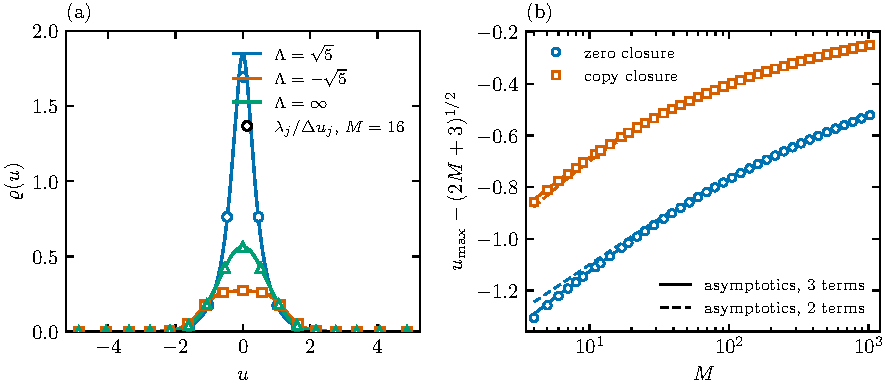
\includegraphics[width=\textwidth]{spectrum}
  \caption{(a) The spectral density $\varrho(u)$ of (\ref{eq:varrho}) for $\Lambda=\sqrt5$, $-\sqrt5$ and $\infty$ (lines), and the Gauss weights $\lambda_j$ of GANDALF's ladder matrix at $M=16$ with the zero closure, divided by the node spacing $\Delta u_j=(u_{j+1}-u_{j-1})/2$, at the nodes $u_j$ (markers in the colour of each line). (b) The largest phase velocity $u_{\max}$ of GANDALF's ladder matrix at $\Lambda=\sqrt5$, minus $(2M+3)^{1/2}$, for $M=4$ to $1024$ with the zero closure (circles) and the copy closure (squares), and the three-term (solid) and two-term (dashed) asymptotic forms (\ref{eq:umax}).}
  \label{fig:spectrum}
\end{figure}

In figure~\ref{fig:spectrum}(a), $\int\varrho\,\dd u=1/p_0$ to round-off, and by (\ref{eq:gauss}) $\lambda_j/\Delta u_j$ approximates $\varrho(u_j)$; for GANDALF's ladder matrix at $M=16$ the two differ on $|u_j|<3$ by at most 8.2\%, 1.8\% and 0.47\% for $\Lambda=\sqrt5$, $-\sqrt5$ and $\infty$. In figure~\ref{fig:spectrum}(b) the three-term forms (\ref{eq:umax}) follow the largest eigenvalue of GANDALF's ladder matrix down to $M=4$ for both closures, and it does not depend on $\Lambda$ to round-off.

\subsection{Slices in a turbulent run}\label{num:snapshots}

\begin{figure}[t]
  \centering
  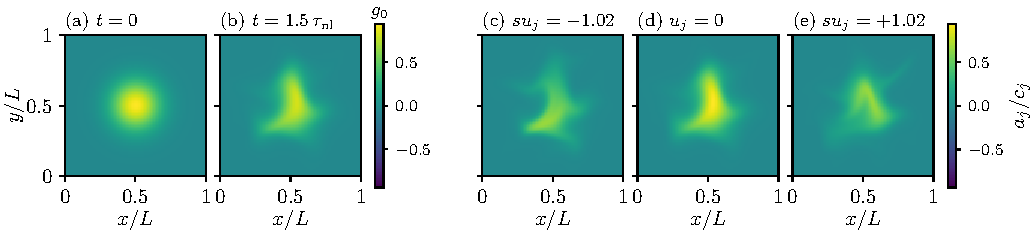
\includegraphics[width=\textwidth]{snapshots}
  \caption{A density blob in decaying Alfv\'enic turbulence, on the plane $z=0$ (coordinates in units of the box side $L=1$). (a, b) The density moment $g_0$ at $t=0$ and $t=1.5\,\tau_{\rm nl}$. (c--e) Three of the 17 slices $a_j$ of the run (section~\ref{sl:transformsec}) at $t=1.5\,\tau_{\rm nl}$, with $su_j=-1.0218$, $u_j=0$ and $su_j=+1.0218$; their stream functions $\Phi+su_j\Psi$ are mainly $z^-$, $\Phi$ alone and mainly $z^+$. At $t=0$ each slice is a constant multiple $c_jf$ of the blob $f$, and the panels show $a_j/c_j$, so all three started as panel (a). They differ at $t=1.5\,\tau_{\rm nl}$ because each was carried by its own flow, and $g_0$ in (b) is a weighted sum of all 17 slices. Panels (c) and (e) are also fainter than (d), because those slices stream along $z$ at $su_j$: the material on their plane $z=0$ started on the planes $z=+0.21$ and $z=-0.21$, where $f$ is about 0.7 of its value at $z=0$. Each group of panels has one symmetric colour scale. GANDALF run on a $64^3$ grid with $M=16$ (zero closure), $\Lambda=\sqrt5$ and $\beta_i=1$; balanced Gaussian random Elsasser fields with $1\le k_\perp/k_1\le3$ and $|k_z|/k_1\le2$, and nonlinearity parameter $\chi=\bar k_\perp z_{\rm rms}/\bar k_\parallel=1.00$, with energy-weighted mean wavenumbers $\bar k_\perp=2.45\,k_1$ and $\bar k_\parallel=1.17\,k_1$ and $z_{\rm rms}=0.478$ the rms of $|\nabla_\perp z^\pm|$; hyper-resistivity damps $z^\pm$ and every $g_m$; no forcing or hypercollisions; $f$ is a Gaussian of standard deviation $1/8$ in $x$ and $y$ and $1/4$ in $z$; $\tau_{\rm nl}=1/(\bar k_\perp z_{\rm rms})=0.1357$ is the outer eddy time.}
  \label{fig:snapshots}
\end{figure}

Figure~\ref{fig:snapshots} releases a density blob, $g(0)=f\,e_0$, into decaying Alfv\'enic turbulence with $\chi=1.00$ and follows the 17 slices of the hierarchy truncated at $M=16$. A density perturbation loads every slice with the same pattern $f$ (section~\ref{sl:forcingsec}). Each slice is then carried by its own stream function $\Phi+su_j\Psi$, which at $su_j=-1.0218$, $0$ and $+1.0218$ is mainly $z^-$, $\Phi$ alone and mainly $z^+$ (proposition~\ref{prop:elsasser}), and streams along $z$ at $su_j$. The three slices end visibly different, and $g_0$ mixes them. The slices keep their values as they are carried: on the plane $z=0$ the peaks of the slices at $su_j=\pm1.0218$ are 0.69 of the initial peak, close to the factor 0.71 by which $f$ falls over their streaming distance of 0.21 along $z$, and the peak of the slice at $u_j=0$ is 0.998 of it. GANDALF's $\partial_tg$ projected on the slices agrees with (\ref{eq:truncslice}), computed with brackets that do not use GANDALF, to $5.2\times10^{-16}$ of the largest slice rate, while the bracket term is 0.56 to 2.2 times the streaming term, and advecting every slice by $\Phi$ alone gives relative errors of 0.30 to 1.46. Over the run each slice energy changes only by the hyper-resistive loss of that slice, to $1.2\times10^{-6}$ of its initial energy, so no free energy passes between slices.

\subsection{The Hermite spectrum of decorrelated slices}\label{num:dictionary}

By section~\ref{dec:sec-dictionary}, the steady state of forced linear phase mixing is the spectrum of $\delta$-correlated slices with $e\propto\varrho$. We computed the steady state of one Fourier mode whose $g_0$ is driven by white noise from GANDALF's ladder matrix at $M=600$, with the outgoing closure $g_{M+1}=-\ii\,\mathrm{sgn}(k_z)\,g_M$ (the closure of \citealt[eq.~4.36]{Kanekar2015} with their $R_{M+1}=1$) and the Lyapunov equation for the steady covariance, and the spectrum of $\delta$-correlated slices from (\ref{eq:dictionary}) by Gauss quadrature. At $\Lambda=\infty$ the forced spectrum differs from the closed form (\ref{eq:prefactor}) by at most $3.1\times10^{-4}$, and at $\Lambda=\sqrt5$ and $-\sqrt5$ from the spectrum with $e\propto\varrho$ by at most $1.5\times10^{-4}$ and $4.2\times10^{-4}$, the size of the closure error. At $m=1$ it is 4.7\% below $(1-1/\Lambda)$ times its value at $\Lambda=\infty$ for $\Lambda=\sqrt5$ and 5.2\% above it for $\Lambda=-\sqrt5$, so this proportionality holds only at large $m$.

\subsection{Further checks and the scripts}\label{num:rhs}

The other checks cited in sections~\ref{sec:model} to~\ref{sec:truncated} use GANDALF's right-hand side. For random states with $M=2$ to 65, $\Lambda=\pm\sqrt5$ and 3, $\beta_i$ from 0.37 to 1.7 and both closures, its $\partial_tg$ satisfies (\ref{eq:truncslice}) to $2\times10^{-13}$, with brackets several times the streaming term, and fails at order one when the sign of $\{\Psi,\cdot\}$ is reversed. Slices at $su_j=-1$ obey proposition~\ref{prop:elsasser} to $5.5\times10^{-16}$ and $1.6\times10^{-15}$, and translate rigidly when $z^-=0$, to $1.4\times10^{-14}$. The two-slice law (\ref{eq:twoslice}) holds to $5\times10^{-15}$ and the two forms of (\ref{eq:fluxCD}) agree to $5\times10^{-14}$. The forms $Q^{(M)}_\varphi$ are conserved to relative rates of $3.2\times10^{-17}$, whereas $\int a_j^4\,\dd^3r$ changes at relative rates of $4.9\times10^{-4}$ and more, so only the quadratic invariants of section~\ref{sec:invariants} survive Fourier truncation.

The self-checking scripts behind these statements are in the repository \url{https://github.com/anjor/krmhd-research}, in the subfolders \url{continuum/}, \url{truncated/} and \url{dynamics/} of \url{paper/phase-velocity-slices/derivations/}; its subfolder \url{review/} holds re-derivations of the same results that share no code with them. Each script prints PASS or FAIL for every check. Figures~\ref{fig:spectrum} and~\ref{fig:snapshots} and the numbers of section~\ref{num:dictionary} come from the scripts \url{fig_spectrum.py}, \url{fig_snapshots.py} and \url{fig_dictionary.py} in \url{paper/phase-velocity-slices/analysis/}, with the configuration files in \url{paper/phase-velocity-slices/configs/}; the run of figure~\ref{fig:snapshots} is \url{P1_slices-turb_20261014_222456}, made with \url{scripts/run_slices_turbulence.py}.

\section{Discussion}\label{sec:discussion}

The slice decomposition (theorems~\ref{thm:slice} and~\ref{thm:trunc}) holds for $k_\perp\rho_i\to0$, for each branch and for the Laguerre sectors with $l\ge2$, for any smooth Alfv\'enic fields, which may be forced, resistive or prescribed, and without collisions, forcing or spatial dissipation of the compressive distribution except where stated. Without collisions the energy of every slice is conserved, so free energy does not move between phase velocities, and velocity-space transfer is the decorrelation and recorrelation of independent passive scalars by their relative streaming along the perturbed field (proposition~\ref{prop:twoslice}). The invariants fix the distribution of free energy over phase velocity but not the correlations between slices, so they impose no Fj{\o}rtoft-type constraint on this transfer (proposition~\ref{prop:nofjortoft}); this concerns transient solutions, not the forced steady states to which CMM's cascade criterion refers.

The slices also show what an ideal induction equation adds. If the field lines are frozen into $\uE$, the compressive distribution is neither forced nor dissipated in space and the Alfv\'enic fields stay smooth, the solution of (\ref{eq:slice}) is $a_u(t)=\mathcal X_t\,\mathsf S_{sut}\,a_u(0)$, where $\mathsf S_\ell=e^{-\ell\gradpar(0)}$ moves a function a distance $\ell$ along the field lines at $t=0$ and $\mathcal X_t$ relabels it with the flow map of $\uE$: each slice is carried rigidly along the initial field lines at its own speed $su$ and then moved with the flow. This is the Lagrangian linearity of S09 (\S6.3), which \citet{Kunz2015} restated for pressure-anisotropic plasmas. Because the flow map preserves volume, every volume-integrated single-point statistic, $W(m)$ and the slice correlations $C(u,u')$ among them, then evolves as in linear phase mixing along the initial field lines, and with forcing that is white in time its mean is a sum of such responses. \citet{KanekarPrep} proves this frozen-line theorem from the kinetic equation (\ref{eq:branch}) directly, without the slices, and uses it to model the Hermite spectrum of forced turbulence. Stochastic echoes in $W(m)$ therefore require a non-ideal induction equation, spatial dissipation of the compressive distribution, forcing correlated in time, or, as the resistivity goes to zero, a failure of flux freezing for fields that do not stay smooth \citep{Eyink2013,Eyink2018,Jafari2026}; the simulations in which echoes were reported \citep{Meyrand2019} dissipate both the magnetic field and the compressive distribution in space, so the theorem does not contradict them.

For simulations, the slices give three practical consequences. An explicit time step for the nonlinear terms must resolve the advection speed of the fastest slice, $su_{\max}|\nabla_\perp\Psi|$ with $u_{\max}$ of (\ref{eq:umax}), not $s|\nabla_\perp\Psi|$ (section~\ref{sec:truncated}). The $M+1$ slice energies are separately conserved by the nonlinear terms, to round-off for states inside the dealiasing band, which gives $M+1$ checks of a code's brackets in place of the single check that conservation of the free energy provides (section~\ref{sec:numerics}). Fluxes and splits of the free energy should be computed along the perturbed field rather than from $k_z$, because a split by the sign of $k_z$ exchanges phase mixing and unmixing on modes whose $k_z$ and field-aligned wavenumber have opposite signs, and diagnostics of the phase-space helicity should use an odd truncation order $M$, for which the conserved discrete helicity is CMM's $\Hph$ on the retained moments (\ref{eq:Hoddeven}). Each slice could also be advanced as an independent passive scalar, for example by a semi-Lagrangian method along its velocity $\boldsymbol U_u$ (\ref{eq:Uu}); we have not tested such a scheme.

In turbulence the compressive distribution is dissipated at small perpendicular scales. Each slice is a passive scalar, and in turbulent flows the rate at which the variance of a passive scalar is dissipated remains finite as the diffusivity goes to zero \citep{ShraimanSiggia2000,FalkovichGawedzkiVergassola2001}. The perpendicular sink of each slice therefore need not disappear as the dissipation coefficients go to zero, and its competition with phase mixing, rather than an ideal echo, may set the Hermite spectrum at large $m$; \citet{KanekarPrep} builds a model of the Hermite spectrum on this competition and tests it in simulations. At finite $k_\perp\rho_i$ the Landau coupling depends on the wavenumber (CMM's 3.10 and 3.14), the advection depends on $v_\perp$ (their 3.16) and the compressive fluctuations act back on the Alfv\'enic ones, so the slices no longer decouple; CMM do not list $\Gamma^\pm$ among the invariants of general gyrokinetics, \citet{CostelloPlunk2025} have extended an invariant of the model of \citet{Plunk2015} to finite Larmor radius, and which invariants survive is open. Velocity-dependent collisions are the only terms that exchange free energy between slices, through the kernel in (\ref{eq:sliceforcing}); how this combines with their decorrelation in turbulence is also open.

% Acknowledgements and any AI-use disclosure to be written by the author.


\appendix
% Appendix equations are numbered (A1), (A2), ... within each appendix.
\counterwithin*{equation}{section}
\renewcommand{\theequation}{\thesection\arabic{equation}}
\renewcommand{\theHequation}{\thesection.\arabic{equation}}
\section{The two compressive branches}\label{app:branches}

We derive the branches of section~\ref{mod:branches} following S09 (\S6.2) and CMM (appendix~B), with $\delta_n\equiv\delta n/n$, $\delta_B\equiv\delta B/B$ and $\langle\cdot\rangle$ the volume average. We checked every identity symbolically, and the moments and splits also by quadrature over $(v_\perp,v_\parallel)$ for random distribution functions.

\subsection{Laguerre projection and the branches}\label{appA:branches}

With $x=v_\perp^2/\vth^2$, CMM (eq.~B8) and S09 (eq.~205) write
\begin{equation*}
  g=\frac{n_i}{\pi\vth^2}\,e^{-x}\sum_{l\ge0}L_l(x)\,G_l(v_\parallel),\qquad
  F_0=\frac{n_i}{\pi\vth^2}\,e^{-x}F_M(v_\parallel),
\end{equation*}
with $L_l$ orthonormal with weight $e^{-x}$ on $(0,\infty)$. Since $x=L_0-L_1$ and $x^k\perp L_l$ for $l>k$, the source term of (\ref{mod:kinetic}) projects only on $L_0$ and $L_1$, and (\ref{mod:kinetic}) and (\ref{mod:fields}) become
\begin{gather*}
  \frac{\dd G_0}{\dd t}+v_\parallel\gradpar\Big[G_0+F_M\Big(\frac{Z}{\tau}\delta_n+\delta_B\Big)\Big]=0,\qquad
  \frac{\dd G_1}{\dd t}+v_\parallel\gradpar\big(G_1-F_M\delta_B\big)=0,\\
  \frac{\dd G_l}{\dd t}+v_\parallel\gradpar G_l=0\quad(l\ge2),\\
  \int G_0\,\dd v_\parallel=\delta_n-\delta_B,\qquad
  \int(G_0-G_1)\,\dd v_\parallel=-\frac{Z}{\tau}\delta_n-2\Big(1+\frac{1}{\beta_i}\Big)\delta_B .
\end{gather*}
With $D=Z/\tau+2(1+\beta_i^{-1})$, the distributions of CMM's eqs~(B2)--(B3) (S09 eqs~176--177),
\begin{equation*}
  G_n=-\frac{1}{D}\Big[(G_0-G_1)-2\Big(1+\frac{1}{\beta_i}\Big)G_0\Big],\qquad
  G_B=-\frac{1}{D}\Big[(G_0-G_1)+\frac{Z}{\tau}G_0\Big],
\end{equation*}
have $\int G_n\,\dd v_\parallel=\delta_n$ and $\int G_B\,\dd v_\parallel=\delta_B$, invert to
\begin{equation}\label{appA:G01}
  G_0=G_n-G_B,\qquad G_1=\Big(1+\frac{Z}{\tau}\Big)G_0+D\,G_B ,
\end{equation}
and obey S09's eqs~(179)--(180),
\begin{equation*}
  \frac{\dd}{\dd t}\begin{pmatrix}G_n\\ G_B\end{pmatrix}+v_\parallel\gradpar\begin{pmatrix}G_n\\ G_B\end{pmatrix}
  =v_\parallel F_M\,\gradpar\,K\begin{pmatrix}\delta_n\\ \delta_B\end{pmatrix},\qquad
  K=\frac{1}{D}\begin{pmatrix}-\dfrac{Z}{\tau}\Big(1+\dfrac{2}{\beta_i}\Big) & -\dfrac{2}{\beta_i}\\[10pt]
  \dfrac{Z}{\tau}\Big(1+\dfrac{Z}{\tau}\Big) & 2+\dfrac{Z}{\tau}\end{pmatrix}.
\end{equation*}
If $\ell K=\Lambda^{-1}\ell$, then $G=\ell\cdot(G_n,G_B)$ has $\int G\,\dd v_\parallel=\ell\cdot(\delta_n,\delta_B)$ and obeys (\ref{mod:Gpm}). The two left eigenvectors give CMM's branches (B5)--(B6) (S09 eqs~183--184),
\begin{equation*}
  G^+=G_B+\frac{1+Z/\tau}{\sigma}\,G_n,\qquad
  G^-=G_n+\frac{2\tau}{\sigma Z\beta_i}\,G_B,\qquad
  \sigma=1+\frac{\tau}{Z}+\frac{1}{\beta_i}+\Delta,
\end{equation*}
and the eigenvalues are $1/\Lambda^\pm$ with $\Lambda^\pm$ and $\Delta$ of (\ref{eq:Lambdapm}).

\subsection{Moments}\label{appA:moments}

The map $(G_n,G_B)\mapsto(G^+,G^-)$ has determinant $-2\Delta/\sigma\ne0$ and inverse
\begin{equation}\label{appA:inv}
  G_n=\frac{\sigma G^--(2\tau/Z\beta_i)\,G^+}{2\Delta},\qquad
  G_B=\frac{\sigma G^+-(1+Z/\tau)\,G^-}{2\Delta},
\end{equation}
so that, with $M_0^\pm=\int G^\pm\,\dd v_\parallel$,
\begin{equation}\label{appA:dndB}
  \delta_n=\frac{\sigma M_0^--(2\tau/Z\beta_i)\,M_0^+}{2\Delta},\qquad
  \delta_B=\frac{\sigma M_0^+-(1+Z/\tau)\,M_0^-}{2\Delta}.
\end{equation}
These are one half of the right-hand sides of S09's eqs~(202)--(203), as CMM found (footnote to their eq.~B15). The parallel flow and pressure perturbations of the non-Alfv\'enic part $g_i=g+x\,\delta_BF_0$ of the ion distribution (CMM eq.~3.26) are
\begin{equation*}
  u_\parallel=\int v_\parallel G_0\,\dd v_\parallel,\qquad
  \frac{\delta p_\perp}{p}=-\frac{Z}{\tau}\delta_n-\frac{2}{\beta_i}\delta_B,\qquad
  \frac{\delta p_\parallel}{p}=\frac{2}{\vth^2}\int v_\parallel^2G_0\,\dd v_\parallel+\delta_B,
\end{equation*}
with $p=n_iT_i$. By (\ref{appA:G01}) and (\ref{appA:inv}) these are linear in $G^\pm$, and the $G_l$ with $l\ge2$ enter only moments $\int\dd^3v\,v_\parallel^jv_\perp^{2k}g_i$ with $k\ge2$.

\subsection{Free energy}\label{appA:energy}

With $x=L_0-L_1$, the orthonormality of the $L_l$ and the field relations, CMM's compressive free energy (their eq.~3.31) becomes
\begin{align*}
  W_{\rm compr}&=\frac{n_iT_i}{2}\Big\langle\frac{Z}{\tau}\delta_n^2+\frac{2}{\beta_i}\delta_B^2
  +\frac{1}{n_i}\int\dd^3v\,\frac{g_i^2}{F_0}\Big\rangle\\
  &=\frac{n_iT_i}{2}\Big\langle\int\frac{G_0^2+G_1^2}{F_M}\,\dd v_\parallel
  +\frac{Z}{\tau}\delta_n^2-\frac{2Z}{\tau}\delta_n\delta_B-2\Big(1+\frac{1}{\beta_i}\Big)\delta_B^2
  +\sum_{l\ge2}\int\frac{G_l^2}{F_M}\,\dd v_\parallel\Big\rangle .
\end{align*}
The part with $l=0,1$ splits between the branches by the identities
\begin{equation}\label{appA:local}
  G_0^2+G_1^2=c_+\,(G^+)^2+c_-\,(G^-)^2,\qquad
  \frac{Z}{\tau}\delta_n^2-\frac{2Z}{\tau}\delta_n\delta_B-2\Big(1+\frac{1}{\beta_i}\Big)\delta_B^2
  =-c_+\frac{(M_0^+)^2}{\Lambda^+}-c_-\frac{(M_0^-)^2}{\Lambda^-},
\end{equation}
the first of which holds at each $v_\parallel$, with
\begin{equation}\label{appA:cpm}
  c_+=\Big[1+\frac{1+\tau/Z}{\Delta}\Big](\Lambda^+)^2>0,\qquad
  c_-=\frac{Z^2}{2\tau^2}\Big[1+\frac{1}{\Delta\beta_i}\Big](\Lambda^-)^2>0 .
\end{equation}
This gives CMM's eq.~(B15) with their eqs~(B13)--(B14),
\begin{equation}\label{appA:split}
  W_{\rm compr}=\tilde W_{\rm compr}+c_+W^+_{\rm compr}+c_-W^-_{\rm compr},\qquad
  W^\pm_{\rm compr}=\frac{n_iT_i}{2}\Big\langle\int\frac{(G^\pm)^2}{F_M}\,\dd v_\parallel-\frac{(M_0^\pm)^2}{\Lambda^\pm}\Big\rangle,
\end{equation}
with $\tilde W_{\rm compr}$ the part with $l\ge2$. Each part is conserved (S09, \S\S6.2.3 and~6.2.5; CMM eq.~B12) and positive definite (section~\ref{sec:slices}).

The coefficients (\ref{appA:cpm}) use $\Delta$ of (\ref{eq:Lambdapm}) (S09 eq.~204) and are one quarter of those in S09's eq.~(213), as CMM state. CMM's eq.~(B16) prints this square root as $[(1+\tau/Z)+\beta_i^{-2}]^{1/2}$, which gives $\sqrt3$ instead of $\sqrt5$ at $\beta_i=\tau=Z=1$. Their eqs~(B6)--(B7) are correct, so the misprint affects only $c_\pm$ in (B15) and (B17) and our (\ref{appA:split}), which then fails. For random distribution functions the relative error in $W_{\rm compr}$ with the printed square root is up to $7.2\times10^{-2}$ over the parameters we tried ($2.5\times10^{-2}$ at $\beta_i=\tau=Z=1$), and below $5\times10^{-14}$ with the square restored.

\section{The slice transform and the spectral theory of the branch operator}\label{app:spectral}

\subsection{Definitions and statement}\label{appB:defs}

Let $\mathcal W$ be the space of real functions $G(u)$ with $\ip{G}{G}<\infty$, where $\ip{f}{g}=\int fg\,F_M^{-1}\,\dd u$, so that $\mathsf Q=F_M\,M_0$ is the orthogonal projector onto $F_M$. The free-energy product (\ref{eq:fe}) is $\fe{f}{g}=\ip{f}{Pg}$ with $P=I-\mathsf Q/\Lambda$, and with $G=M_0[G]\,F_M+G_\perp$, $\fe{G}{G}=\ip{G_\perp}{G_\perp}+p_0\,M_0[G]^2$, which is positive definite, with a norm equivalent to that of $\ip{\cdot}{\cdot}$, if and only if $\Lambda\notin[0,1]$. With $U$ the multiplication by $u$,
\begin{equation}\label{eq:LUP}
  L=UP ,
\end{equation}
so $\fe{f}{Lg}=\ip{Pf}{UPg}$ is symmetric in $f$ and $g$. For $\mathrm{Im}\,z>0$,
\begin{equation}\label{sl:resolvent}
  (z-L)^{-1}G=\frac{1}{z-u}\left[G-\frac{uF_M}{\Lambda\,\diel(z)}\int\frac{G(v)}{z-v}\,\dd v\right],\qquad
  \diel(\zeta)=1-\frac{1+\zeta Z(\zeta)}{\Lambda},
\end{equation}
where $Z$ is the plasma dispersion function of \citet{FriedConte1961}, not the charge number; we write $\diel$ also for its continuation into the lower half plane, whose zeros are the Landau roots. On the real axis
\begin{equation}\label{sl:epsRI}
  \diel(u+\ii0)=\diel_R(u)+\ii\,\diel_I(u),\qquad
  \diel_R=1-\frac{1+u\,\mathrm{Re}\,Z(u)}{\Lambda},\qquad
  \diel_I=-\frac{\pi\,u\,F_M(u)}{\Lambda},
\end{equation}
and $\mathsf H[f](u)=\pi^{-1}\PVint f(v)\,(v-u)^{-1}\,\dd v$. By the argument of \citet{Penrose1960}, $\diel$ has no zeros in the closed upper half plane for $\Lambda\notin[0,1]$ (section~\ref{appB:penrose}). The spectral density
\begin{equation}\label{eq:varrho}
  \varrho(u)=\frac{F_M(u)}{|\diel(u+\ii0)|^2}
\end{equation}
is then positive, smooth and even, with $\int\varrho\,\dd u=1/p_0$. For real $u$ the equation $(L-u)F=0$ has the Case--Van Kampen solutions
\begin{equation}\label{sl:Fu}
  F_u(v)=\frac{1}{\Lambda}\,\mathrm P\frac{vF_M(v)}{v-u}+\diel_R(u)\,\delta(v-u),\qquad M_0[F_u]=1,\qquad M_1[F_u]=u,
\end{equation}
and the slice transform is the projection on them in the free-energy product,
\begin{equation}\label{eq:transform}
  \Tr[G](u)=\fe{F_u}{G}=\frac{\diel_R\,G-\diel_I\,\mathsf H[G]}{F_M}(u),\qquad \Tr[LG](u)=u\,\Tr[G](u),
\end{equation}
of which the slice amplitude (\ref{eq:aunit}) is the unit-weight form, $a_u=\sqrt{\varrho(u)}\,\Tr[G](u)$; $\mathcal A$ denotes the map $G\mapsto a$.

\begin{theorem}\label{thm:spectrum}
Let $\Lambda\notin[0,1]$, the value $\Lambda=\infty$ included. Then $L$, with the domain $D(U)$ of $U$, is self-adjoint in $(\mathcal W,\fe{\cdot}{\cdot})$; it has no eigenvalues, and its spectrum is the real line, purely absolutely continuous and simple; and $\mathcal A$ is a unitary map from $(\mathcal W,\fe{\cdot}{\cdot})$ onto $L^2(\mathbb R,\dd u)$ with $\mathcal ALG=u\,\mathcal AG$ for $G\in D(U)$. In particular (\ref{sl:parseval}) holds, $\fe{G}{\varphi(L)G}=\int\varphi(u)\,a_u^2\,\dd u$ for every bounded Borel function $\varphi$, and
\begin{equation}\label{sl:inverse}
  G=\int\varrho(u)\,\Tr[G](u)\,F_u\,\dd u=\diel_R\,c+\diel_I\,\mathsf H[c],\qquad c=\sqrt\varrho\;a .
\end{equation}
\end{theorem}

The rest of this appendix proves the theorem and the statements about the eigenvalues of $L$ and the zeros of $\diel$. For $0<\Lambda<1$, $\diel$ has one zero in the upper half plane, on the imaginary axis, $L$ has the eigenvalues $\pm\ii\gamma$, and the slice decomposition is incomplete.

\subsection{Preliminaries}\label{appB:prelim}

We work in the complexification of $\mathcal W$, with $\ip{f}{g}=\int\bar f\,g\,F_M^{-1}\,\dd u$. The set $\mathcal D_0$ of functions $pF_M$, with $p$ a polynomial, is dense in $\mathcal W$ (it contains the orthonormal basis $e_m$), lies in $D(U)$, and is mapped into itself by $U$, $P$ and $L$. Let $\mathcal S$ be the set of smooth $f$ with $|f(v)|\le C(1+|v|)^kF_M(v)$ for some $C$ and $k$; it contains $\mathcal D_0$ and the smooth functions with compact support. For $f\in\mathcal S$ the Cauchy integral
\begin{equation*}
  \chi_f(\zeta)=\frac{1}{\pi}\int\frac{f(v)}{v-\zeta}\,\dd v\qquad(\mathrm{Im}\,\zeta>0)
\end{equation*}
is analytic in the upper half plane, extends continuously to the real axis with $\chi_f(u+\ii0)=\mathsf H[f](u)+\ii f(u)$ (the Plemelj formula), and is $O(1/\zeta)$ as $|\zeta|\to\infty$ in the closed upper half plane. The following converse is used twice.

\begin{lemma}\label{appB:lemma}
Let $Y$ be analytic in the upper half plane, continuous up to the real axis, and $O(1/\zeta)$ as $|\zeta|\to\infty$ in the closed upper half plane. Then $Y=\chi_y$ with $y(u)=\mathrm{Im}\,Y(u+\ii0)$.
\end{lemma}

\begin{proof}
For $\mathrm{Im}\,\zeta>0$, Cauchy's formula on a large half disc gives $Y(\zeta)=(2\pi\ii)^{-1}\int Y(v+\ii0)\,(v-\zeta)^{-1}\,\dd v$, and Cauchy's theorem for $\overline{Y(\bar\zeta)}$, analytic in the lower half plane with the same decay, gives $\int\overline{Y(v+\ii0)}\,(v-\zeta)^{-1}\,\dd v=0$. Subtracting $(2\pi\ii)^{-1}$ times the second integral from the first gives $Y=\chi_y$.
\end{proof}

\subsection{Self-adjointness}\label{appB:sa}

Let $\Lambda\notin[0,1]$, so that $p_0>0$. Since $P=(I-\mathsf Q)+p_0\mathsf Q$, the operator $P^{1/2}=I+(\sqrt{p_0}-1)\mathsf Q$ is bounded and symmetric, with bounded inverse, and $\fe{f}{g}=\ip{P^{1/2}f}{P^{1/2}g}$, so $V:G\mapsto P^{1/2}G$ is unitary from $(\mathcal W,\fe{\cdot}{\cdot})$ onto $(\mathcal W,\ip{\cdot}{\cdot})$. Since $V-I$ has its range in the span of $F_M\in D(U)$, $V$ maps $D(U)$ onto itself, and by (\ref{eq:LUP})
\begin{equation}\label{appB:rank2}
  VLV^{-1}=P^{1/2}UP^{1/2}=U+\mathsf K,\qquad
  \mathsf K=(\sqrt{p_0}-1)\big(\mathsf QU+U\mathsf Q\big),
\end{equation}
where $(\sqrt{p_0}-1)^2\mathsf QU\mathsf Q$ is absent because $\mathsf QU\mathsf QG=M_1[F_M]\,M_0[G]\,F_M=0$. The operator $\mathsf KG=(\sqrt{p_0}-1)\big[\ip{uF_M}{G}\,F_M+\ip{F_M}{G}\,uF_M\big]$ is symmetric, of rank two and bounded, since $\ip{F_M}{F_M}=1$ and $\ip{uF_M}{uF_M}=1/2$. By the Kato--Rellich theorem \citep[][chapter~V]{Kato1966}, $U+\mathsf K$ is then self-adjoint on $D(U)$ in $(\mathcal W,\ip{\cdot}{\cdot})$, so $L=V^{-1}(U+\mathsf K)V$ is self-adjoint on $D(U)$ in $(\mathcal W,\fe{\cdot}{\cdot})$, which is part~(i) of theorem~\ref{thm:spectrum}.

\subsection{Eigenvalues}\label{appB:eig}

For every $\Lambda\neq0$, a function $G\in D(U)$ is an eigenfunction of $L$ with eigenvalue $\lambda$ if and only if
\begin{equation*}
  (u-\lambda)\,G=\frac{uF_M}{\Lambda}\,M_0[G],\qquad G\neq0 .
\end{equation*}
If $\lambda$ is not real, $G=M_0[G]\,uF_M/[\Lambda(u-\lambda)]$, and taking $M_0$ gives $M_0[G]\,\diel(\lambda)=0$ if $\mathrm{Im}\,\lambda>0$ and $M_0[G]\,\overline{\diel(\bar\lambda)}=0$ if $\mathrm{Im}\,\lambda<0$, because the integral in (\ref{sl:resolvent}) at a point of the lower half plane equals $\overline{\diel(\bar\lambda)}$ (for the same reason the resolvent for $\mathrm{Im}\,z<0$ is (\ref{sl:resolvent}) with $\overline{\diel(\bar z)}$ in place of $\diel(z)$). Since $M_0[G]=0$ would give $G=0$, a non-real $\lambda$ is an eigenvalue if and only if $\lambda$ or $\bar\lambda$ is a zero of $\diel$ in the upper half plane. For real $\lambda\neq0$, $uF_M/(u-\lambda)$ is not square integrable near $u=\lambda$, so $M_0[G]=0$ and $G=0$. For $\lambda=0$, $G=M_0[G]\,F_M/\Lambda$ requires $\Lambda=1$.

\subsection{Zeros of the dielectric function}\label{appB:penrose}

The function $\diel$ is analytic in the upper half plane and continuous up to the real axis, where it takes the values (\ref{sl:epsRI}). Since $1+\zeta Z(\zeta)=-1/(2\zeta^2)+O(\zeta^{-4})$ uniformly in $\mathrm{Im}\,\zeta\ge0$, $\diel\to1$ as $|\zeta|\to\infty$ there, so if $\diel$ has no real zeros, the number of its zeros in the upper half plane is the winding number about $0$ of the closed curve $u\mapsto\diel(u+\ii0)$. A real zero requires $\diel_I(u)=0$, hence $u=0$, and $\diel_R(0)=p_0$ vanishes only at $\Lambda=1$. For $\Lambda\neq1$, $\diel(u+\ii0)=1-\mathcal N(u)/\Lambda$ with $\mathcal N(u)=1+uZ(u+\ii0)$, and the winding number of $\diel$ about $0$ equals that of $\mathcal N$ about the point $\Lambda$. The curve $\mathcal N$ has $\mathrm{Im}\,\mathcal N(u)=\pi uF_M(u)$, $\mathcal N(0)=1$ and $\mathcal N(u)\to0$ as $|u|\to\infty$: it leaves $0$ at $u=-\infty$, runs through the lower half plane to the point $1$, reached at $u=0$, and returns to $0$ through the upper half plane, meeting the real axis only at $0$ and $1$. It therefore winds once around every point of $(0,1)$ and around no real point outside $[0,1]$, so
\begin{equation}\label{appB:count}
  \#\{\zeta:\ \diel(\zeta)=0,\ \mathrm{Im}\,\zeta\ge0\}=
  \begin{cases}0, & \Lambda<0\ \text{or}\ \Lambda>1,\\ 1, & 0<\Lambda<1,\end{cases}
\end{equation}
which is the criterion of \citet{Penrose1960} for this dielectric function. By section~\ref{appB:eig}, $L$ has no eigenvalues for $\Lambda\notin[0,1]$.

The plasma dispersion function continues to the entire function $Z(\zeta)=\ii\sqrt\pi\,e^{-\zeta^2}\mathrm{erfc}(-\ii\zeta)$, and the zeros of the continued $\diel$ in the lower half plane are the Landau roots. They are not eigenvalues of $L$, because in the lower half plane the resolvent contains $\overline{\diel(\bar\zeta)}$, which by (\ref{appB:count}) has no zeros there for $\Lambda\notin[0,1]$.

\subsection{Spectral measure}\label{appB:stone}

For $\mathrm{Im}\,z>0$ and real $G\in\mathcal W$, let
\begin{equation*}
  C_G(z)=\int\frac{G(v)}{z-v}\,\dd v,\qquad I_G(z)=\int\frac{G(v)^2}{(z-v)\,F_M(v)}\,\dd v .
\end{equation*}
By (\ref{sl:resolvent}), $M_0[(z-L)^{-1}G]=C_G(z)/\diel(z)$, and since $\int uG(u)\,(z-u)^{-1}\,\dd u=zC_G(z)-M_0[G]$, the resolvent form is
\begin{equation*}
  R_G(z)\equiv\fe{G}{(z-L)^{-1}G}=I_G(z)-\frac{z}{\Lambda}\,\frac{C_G(z)^2}{\diel(z)} .
\end{equation*}
It is the Stieltjes transform $\int(z-x)^{-1}\,\dd\mu_G(x)$ of the spectral measure $\mu_G$ of $L$ in the state $G$, which Stone's formula recovers:
\begin{equation}\label{appB:stoneformula}
  \mu_G\big((u_1,u_2)\big)+\tfrac12\mu_G\big(\{u_1\}\big)+\tfrac12\mu_G\big(\{u_2\}\big)
  =-\frac{1}{\pi}\lim_{\eta\to0+}\int_{u_1}^{u_2}\mathrm{Im}\,R_G(u+\ii\eta)\,\dd u .
\end{equation}

Let $G\in\mathcal D_0$ be real and $\Lambda\notin[0,1]$. Then $C_G=-\pi\chi_G$ and $I_G=-\pi\chi_{G^2/F_M}$ extend continuously to the real axis, with $C_G(u+\ii0)=-\pi(\mathsf H[G]+\ii G)(u)$ and $\mathrm{Im}\,I_G(u+\ii0)=-\pi G(u)^2/F_M(u)$. By (\ref{appB:count}), $1/\diel$ is continuous on the closed upper half plane, so $R_G(u+\ii\eta)\to R_G(u+\ii0)$ as $\eta\to0+$, uniformly for $u$ in compact sets. With $\diel_I=-\pi uF_M/\Lambda$, the imaginary part of the boundary value is a square:
\begin{equation*}
  -\frac{1}{\pi}\,\mathrm{Im}\,R_G(u+\ii0)
  =\frac{G^2}{F_M}-\frac{\diel_I}{F_M}\,\frac{2\diel_R\,G\,\mathsf H[G]-\diel_I\big(\mathsf H[G]^2-G^2\big)}{|\diel|^2}
  =\frac{\big(\diel_RG-\diel_I\mathsf H[G]\big)^2}{F_M\,|\diel|^2}
  =\varrho\,\Tr[G]^2=a_u^2 .
\end{equation*}
By (\ref{appB:stoneformula}) and the uniform convergence, $\mu_G$ has no atoms and $\dd\mu_G=a_u^2\,\dd u$.

Three consequences follow. First, the absolutely continuous subspace of $L$ is closed and contains the dense set $\mathcal D_0$, so it is $\mathcal W$, and $L$ has no eigenvalues and no singular continuous spectrum. Second, $\mathsf K$ in (\ref{appB:rank2}) has rank two and is therefore of trace class, so by the Kato--Rosenblum theorem \citep[][chapter~X]{Kato1966} the absolutely continuous parts of $U+\mathsf K=VLV^{-1}$ and of $U$ are unitarily equivalent; since both operators are purely absolutely continuous, $L$ is unitarily equivalent to $U$, multiplication by $u$ in $L^2(\mathbb R,\dd u/F_M)$, whose spectrum is the real line with multiplicity one. This is part~(ii) of theorem~\ref{thm:spectrum}. Third, applying $\dd\mu_G=a_u^2\,\dd u$ to $G+G'$ and $G-G'$ gives, for real $G,G'\in\mathcal D_0$ and every bounded Borel function $\varphi$,
\begin{equation}\label{appB:polar}
  \fe{G'}{\varphi(L)G}=\int\varphi(u)\,a_u[G']\,a_u[G]\,\dd u,\qquad a[G]=\mathcal AG ,
\end{equation}
and by linearity the same holds for complex $G,G'\in\mathcal D_0$ with $a_u[G']$ replaced by its complex conjugate.

\subsection{The slice transform}\label{appB:transform}

The formula (\ref{eq:aunit}), with $\mathsf H$ the Hilbert transform on $L^2(\mathbb R,\dd u)$, defines a bounded operator $\mathcal A$ from $\mathcal W$ into $L^2(\mathbb R,\dd u)$: for $\Lambda\notin[0,1]$, $|\diel(u+\ii0)|$ is bounded below, since it has no real zeros and tends to $1$ at infinity, and since $|\diel_R|\le|\diel|$, the first term of (\ref{eq:aunit}) has norm at most $\ip{G}{G}^{1/2}$. In the second, $\diel_I\mathsf H[G]/(\sqrt{F_M}\,|\diel|)=-\pi u\sqrt{F_M}\,\mathsf H[G]/(\Lambda|\diel|)$, the factor $u\sqrt{F_M}/|\diel|$ is bounded, $\mathsf H$ is an isometry, and $\int|G|^2\,\dd u\le\pi^{-1/2}\ip{G}{G}$. By (\ref{appB:polar}) with $\varphi=1$, $\mathcal A$ is isometric on the dense set $\mathcal D_0$, so it is an isometry of $(\mathcal W,\fe{\cdot}{\cdot})$ into $L^2(\mathbb R,\dd u)$, and its range is closed.

The following argument is the counterpart for $L$ of the invertibility proof of \citet{Morrison2000}. To show that the range of $\mathcal A$ is dense, let $b$ be a smooth function with compact support, $c=\sqrt\varrho\,b$, and
\begin{equation*}
  G=\diel_Rc+\diel_I\mathsf H[c]=\mathrm{Im}\big[\diel(u+\ii0)\,\chi_c(u+\ii0)\big].
\end{equation*}
Since $c$ has compact support, $\diel_I=-\pi uF_M/\Lambda$ and $\mathsf H[c]$ is smooth and bounded, $G$ belongs to $\mathcal S$ and to $\mathcal W$. The product $\diel\chi_c$ is analytic in the upper half plane, continuous up to the real axis and $O(1/\zeta)$, so by lemma~\ref{appB:lemma} it equals $\chi_G$, and $\chi_c(u+\ii0)=\chi_G(u+\ii0)/\diel(u+\ii0)$. Taking imaginary parts, with the Plemelj formula for $\chi_G$,
\begin{equation*}
  c=\frac{\mathrm{Im}\big[(\mathsf H[G]+\ii G)\,\bar\diel\big]}{|\diel|^2}=\frac{\diel_RG-\diel_I\mathsf H[G]}{|\diel|^2}=\varrho\,\Tr[G],
\end{equation*}
so that $\mathcal AG=b$. The smooth functions with compact support are dense in $L^2(\mathbb R,\dd u)$ and the range of $\mathcal A$ is closed, so $\mathcal A$ is onto, with the inverse
\begin{equation}\label{appB:inv}
  \mathcal A^{-1}a=\diel_R\sqrt\varrho\,a+\diel_I\,\mathsf H\big[\sqrt\varrho\,a\big],
\end{equation}
which is (\ref{sl:inverse}): since $|\diel_R|\sqrt{\varrho/F_M}\le1$ and $|\diel_I|/\sqrt{F_M}$ and $\varrho$ are bounded, the right-hand side is a bounded operator from $L^2(\mathbb R,\dd u)$ into $\mathcal W$ that equals $\mathcal A^{-1}$ on a dense set. Conversely, for $G\in\mathcal D_0$, $Y=\chi_G/\diel$ is analytic in the upper half plane, because $\diel$ has no zeros there, and $\mathrm{Im}\,Y(u+\ii0)=\varrho\Tr[G]=c\in\mathcal S$; by lemma~\ref{appB:lemma}, $Y=\chi_c$, and $G=\mathrm{Im}\,\chi_G(u+\ii0)=\mathrm{Im}[\diel\,Y](u+\ii0)=\diel_Rc+\diel_I\mathsf H[c]$. The first direction does not use the zeros of $\diel$ in the upper half plane; the second uses their absence, and fails by the residue of $Y$ at the zero $\ii\gamma$ that $\diel$ has for $0<\Lambda<1$, where $1-\sqrt\pi\,\gamma\,e^{\gamma^2}\mathrm{erfc}(\gamma)=\Lambda$ and $L$ has the eigenvalues $\pm\ii\gamma$ (section~\ref{appB:eig}); the slices are then not complete. The KRMHD branches never fall in this range, because $\Lambda^+>1$ and $\Lambda^-<0$.

Part~(iii) of theorem~\ref{thm:spectrum} follows. By (\ref{appB:polar}) with $\varphi(u)=(z-u)^{-1}$, $\mathrm{Im}\,z\neq0$, $\fe{G'}{(z-L)^{-1}G}=\int\overline{a_u[G']}\,a_u[G]\,(z-u)^{-1}\,\dd u$ for $G,G'\in\mathcal D_0$, and by continuity for all $G,G'\in\mathcal W$. Since $\mathcal A$ is unitary, the left-hand side is $\int\overline{a_u[G']}\,a_u[(z-L)^{-1}G]\,\dd u$, and since $\mathcal AG'$ runs over $L^2(\mathbb R,\dd u)$, $\mathcal A(z-L)^{-1}G=(z-u)^{-1}\mathcal AG$. For $G\in D(U)$, applying this to $(z-L)G$ shows that $u\,\mathcal AG\in L^2(\mathbb R,\dd u)$ and $\mathcal ALG=u\,\mathcal AG$. The relations (\ref{sl:parseval}) are then the functional calculus of multiplication by $u$.

By (\ref{sl:Fu}), $\int c(u)\,F_u(v)\,\dd u=\diel_R(v)\,c(v)+\diel_I(v)\,\mathsf H[c](v)$, so (\ref{appB:inv}) is the completeness relation $G=\int\varrho\,\Tr[G]\,F_u\,\dd u$ of the modes, and $\varrho\,\Tr[\mathcal A^{-1}a]=\sqrt\varrho\,a$ is the orthogonality relation $\fe{F_u}{F_{u'}}=\delta(u-u')/\varrho(u)$, in the sense of distributions.

\section{The truncated hierarchy}\label{app:truncated}

\subsection{Weights, closures and eigenvectors}

Let $J$ be the ladder matrix of the zero closure at $\Lambda=\infty$, the symmetric Jacobi matrix of the Hermite polynomials $h_m$ orthonormal with weight $F_M$, and $J_c$ that of the copy closure, which for $M\ge2$ differs from $J$ only in $(J_c)_{M,M-1}=\sqrt{M/2}+\sqrt{(M+1)/2}$. A finite $\Lambda$ changes only $A_{10}=(1-1/\Lambda)\,J_{10}$, and column $0$ of $J$ and of $J_c$ has the single non-zero entry $J_{10}=1/\sqrt2$. Hence, with $P_\Lambda=\mathrm{diag}(1-1/\Lambda,1,\dots,1)$,
\begin{equation}\label{appC:factor}
  A=J\,P_\Lambda\quad\text{(zero closure)},\qquad A=J_c\,P_\Lambda\quad\text{(copy closure, $M\ge2$)},
\end{equation}
the Hermite form of $L=UP$ (\ref{eq:LUP}). For the zero closure $\Pw=P_\Lambda$, and $\Pw A=P_\Lambda JP_\Lambda$ is symmetric. For the copy closure $D_c=\mathrm{diag}(1,\dots,1,p_M)$ satisfies $D_cJ_c=J$, because $p_M(J_c)_{M,M-1}=\sqrt{M/2}$, so that with $\Pw=D_cP_\Lambda$ again $\Pw A=P_\Lambda JP_\Lambda$.

Since $LF_u=uF_u$ and the untruncated ladder matrix is the matrix of $L$ in the Hermite basis, the Hermite coefficients $r_m(u)$ of $F_u$ satisfy $\sum_nA_{mn}r_n=u\,r_m$ row by row, with $r_0=M_0[F_u]=1$:
\begin{equation}\label{appC:rec}
  r_1=\sqrt2\,u,\qquad r_2=u\,r_1-\frac{1-1/\Lambda}{\sqrt2}\,r_0,\qquad
  \sqrt{\frac{m+1}{2}}\;r_{m+1}=u\,r_m-\sqrt{\frac m2}\;r_{m-1}\quad(m\ge2).
\end{equation}
Thus $r_m$ is a polynomial of degree $m$ with $r_m(-u)=(-1)^mr_m(u)$, and $r_m=h_m$ at $\Lambda=\infty$. Rows $0$ to $M-1$ of the truncated matrix coincide with those of the infinite matrix for both closures, and row $M$ is the condition on the eigenvalues,
\begin{equation}\label{appC:eigcond}
  r_{M+1}(u_j)=0\quad\text{(zero closure)},\qquad r_{M+1}(u_j)=r_{M-1}(u_j)\quad\text{(copy closure)},
\end{equation}
the second from row $M$ of the copy closure, $u\,r_M=[\sqrt{M/2}+\sqrt{(M+1)/2}\,]\,r_{M-1}$, and the recurrence at $m=M$.

\begin{proof}[Proof of theorem~\ref{thm:trunc}]
(i) $A$ is similar to the symmetric tridiagonal matrix $\Pw^{1/2}A\,\Pw^{-1/2}$, whose off-diagonal entries are non-zero because $A_{01}A_{10}=(1-1/\Lambda)/2>0$, so its eigenvalues are real and simple and the vectors $\Pw^{1/2}\boldsymbol r_j$ are orthogonal. By (\ref{appC:rec}) the vector $(r_0(u),\dots,r_M(u))^{\mathsf T}$ satisfies rows $0$ to $M-1$ of $A\boldsymbol r=u\boldsymbol r$ for every $u$, (\ref{appC:eigcond}) fixes the $u_j$, and $\Pw A=A^{\mathsf T}\Pw$ gives $\boldsymbol w_j^{\mathsf T}A=u_j\boldsymbol w_j^{\mathsf T}$. (ii) The combination $\boldsymbol w_j^{\mathsf T}g$ commutes with the brackets, with $\partial_z$ and with the linear operations, and $\boldsymbol w_j^{\mathsf T}A=u_j\boldsymbol w_j^{\mathsf T}$ turns $s\gradpar(Ag)$ into $su_j\gradpar(\boldsymbol w_j^{\mathsf T}g)$; the converse follows from (iii). (iii) By (i), $R^{\mathsf T}\Pw R=I$, so $g=Ra$ and $\sum_mp_m|g_m|^2=a^\dagger R^{\mathsf T}\Pw R\,a=\sum_j|a_j|^2$.
\end{proof}

\subsection{Gauss quadrature}

We prove proposition~\ref{tr:gaussprop}. For the basis functions $e_m$, $\Tr[e_m](u)=\fe{F_u}{e_m}=p_m\,r_m(u)$. (i) By theorem~\ref{thm:spectrum} the slice transform is unitary, and the slice amplitude of $e_m$ is $\sqrt\varrho\,p_mr_m$, so $p_m\delta_{mn}=\fe{e_m}{e_n}=\int\varrho\,p_mr_m\,p_nr_n\,\dd u$. (ii) The polynomials $\sqrt{p_m}\,r_m$ are therefore orthonormal for $\varrho\,\dd u$, with the Jacobi matrix $\Pw^{1/2}A\,\Pw^{-1/2}$ by (\ref{appC:rec}), and the zero closure keeps its first $M+1$ rows and columns. By the theorem of \citet{GolubWelsch1969}, the eigenvalues of this truncated matrix are the zeros of $r_{M+1}$ and the nodes of the Gauss rule, and the weights are $\mu_0O_{0j}^2$, with $O$ its orthonormal eigenvectors and $\mu_0=\int\varrho\,\dd u=1/p_0$. Since $O_{mj}=\sqrt{p_m}\,R_{mj}$, the weights are $R_{0j}^2=1/n_j$, and exactness to degree $2M+1$ is Gauss's theorem. (iii) By definition $\boldsymbol r_j$ holds the Hermite coefficients of $F_{u_j}$, and $\Tr[G](u_j)=\sum_mg_mp_mr_m(u_j)=\boldsymbol w_j^{\mathsf T}g=\sqrt{n_j}\,a_j$.

\subsection{The largest phase velocity}

For the zero closure $A=J+\delta A$ exactly, with $\delta A=-(\Lambda\sqrt2)^{-1}\boldsymbol e_1\boldsymbol e_0^{\mathsf T}$ and $\boldsymbol e_m$ the $m$th unit vector. The eigenvalues of $J$ are the zeros $x_j$ of $h_{M+1}$, and its normalised eigenvectors have components $(\lambda^\infty_j)^{1/2}h_m(x_j)$, with $\lambda^\infty_j$ the Gauss--Hermite weights. Since $h_0=1$ and $h_1(x)=\sqrt2\,x$, to first order $u_j=x_j-\lambda^\infty_jx_j/\Lambda+O(\Lambda^{-2})$. The weight $\lambda^\infty_M$ is of order $e^{-x_M^2}$ up to an algebraic factor, with $x_M^2=2M+3-2^{2/3}|\alpha_1|(2M+3)^{1/3}+\dots$, so the shift of $u_{\max}$ is about $10^{-49}$ at $M=64$. Up to such terms, $u_{\max}$ is the largest zero of $\psi_{M+1}$ for the zero closure and the largest root of $\psi_{M+1}=\psi_{M-1}$ for the copy closure.

The function $\psi_{M+1}$ solves $\psi''+(q^2-x^2)\psi=0$ with $q=q_{M+1}$. With $x=q+(2q)^{-1/3}\xi$ and $\sigma=(2q)^{-4/3}$, the uniform Airy (Langer) approximation $\psi\propto(\chi')^{-1/2}\mathrm{Ai}(\chi)$, with $\chi=\xi+\sigma\xi^2/5+O(\sigma^2)$, places the largest zero at $\chi=\alpha_1$, which gives the first line of (\ref{eq:umax}), the classical expansion of \citet[theorem~6.32]{Szego1975} and \citet{Olver1959} \citep[eq.~12.11.9]{DLMF}. For the copy closure, $x\psi_M=\sqrt{M/2}\,\psi_{M-1}+\sqrt{(M+1)/2}\,\psi_{M+1}$ and $\psi_M'=\sqrt{M/2}\,\psi_{M-1}-\sqrt{(M+1)/2}\,\psi_{M+1}$ turn row $M$, $\psi_{M+1}=\psi_{M-1}$, into the Robin condition $\psi_M'+x(\sqrt M+\sqrt{M+1})^{-2}\psi_M=0$ on $\psi_M$, which solves the same equation with $q=q_M$ and to leading order reads $\psi_\xi+\sigma\psi=0$. The same approximation turns this condition into
\begin{equation*}
  \mathrm{Ai}'(\chi)+\tfrac45\,\sigma\,\mathrm{Ai}(\chi)=0,\qquad\text{so that}\qquad \chi=\alpha_1'-\frac{4\sigma}{5\alpha_1'}+O(\sigma^2),
\end{equation*}
and $\xi=\chi-\sigma\chi^2/5$ gives the second line of (\ref{eq:umax}); $u_{\max}$ up to $M=16384$ confirms both lines.

\subsection{The phase-space helicity at odd and even \texorpdfstring{$M$}{M}}

Since $\PVint F_M\,u^{-1}\,\dd u=0$,
\begin{equation*}
  (B_M)_{mn}=\int\frac{h_m(u)h_n(u)-h_m(0)h_n(0)}{u}\,F_M(u)\,\dd u .
\end{equation*}
The integrand $f_{mn}$ is a polynomial of degree $m+n-1\le2M-1$, so the Gauss--Hermite rule gives $(B_M)_{mn}=\sum_j\lambda^\infty_jf_{mn}(x_j)$ exactly. The nodes come in pairs $\pm x_j$ with equal weights, so $\sum_{x_j\neq0}\lambda^\infty_j/x_j=0$, and $J=O_\infty\,\mathrm{diag}(x_j)\,O_\infty^{\mathsf T}$ with $(O_\infty)_{mj}=(\lambda^\infty_j)^{1/2}h_m(x_j)$. For odd $M$ no node lies at $u=0$, so $(B_M)_{mn}=\sum_j\lambda^\infty_jh_m(x_j)h_n(x_j)/x_j=(J^{-1})_{mn}$, and by (\ref{appC:factor}) $\Pw A^{-1}=J^{-1}$ for every $\Lambda\neq1$; $A$ is invertible because $\det A=(-1)^{(M+1)/2}\prod_{i=0}^{(M-1)/2}A_{2i,2i+1}A_{2i+1,2i}$ vanishes only at $\Lambda=1$. For even $M$ the node $x_{M/2}=0$ contributes $\lambda^\infty_{M/2}f_{mn}(0)=\lambda^\infty_{M/2}[h_m'(0)h_n(0)+h_m(0)h_n'(0)]$ and the other nodes give $(J^+)_{mn}$, which is the second relation of (\ref{eq:Hoddeven}). The conserved form $\Pw A^D$, with the Drazin inverse $A^D$ (eigenvalues $1/u_j$ for $u_j\neq0$ and $0$ at $u=0$), reduces to $J^+$ at $\Lambda=\infty$, so that there $g^{\mathsf T}(\Pw A^D-B_M)g=-2\lambda^\infty_{M/2}[\boldsymbol h(0)\cdot g][\boldsymbol h'(0)\cdot g]$. At finite $\Lambda$, $\Pw A^D\neq J^+$.

For the zero closure and even $M$, $\boldsymbol h(0)$ is a left null vector of $A$ for every $\Lambda$: column $0$ of $\boldsymbol h(0)^{\mathsf T}A$ is $h_1(0)A_{10}=0$, the columns $0<n<M$ vanish by the recurrence $\sqrt{(n+1)/2}\,h_{n+1}(0)+\sqrt{n/2}\,h_{n-1}(0)=0$, and column $M$ is $h_{M-1}(0)\sqrt{M/2}=0$ because $h_{M-1}$ is odd. The $r_m$ and $h_m$ obey the same recurrence for $m\ge2$, and $r_2(0)=p_0h_2(0)$, so $r_m(0)=p_0h_m(0)$ for $m\ge1$ and $\boldsymbol w_{M/2}=\Pw\boldsymbol r_{M/2}=p_0\boldsymbol h(0)$. Hence $a_{M/2}^2=\lambda_{M/2}\,p_0^2\,G_M(0)^2/F_M(0)^2$, with $G_M=\sum_{m\le M}g_me_m$, whose volume average is proportional to the imaginary part of (\ref{eq:Hcomplex}) for the truncated state.

Under the copy closure, $J_c^{-1}=J^{-1}D_c$, so at odd $M$ the conserved form is $g^{\mathsf T}D_cJ^{-1}D_cg$, whose matrix differs from $B_M$ by 33\% at $M=9$ and 23\% at $M=33$, relative to the largest element; at even $M$ the last component of the null vector is multiplied by $p_M$.

\clearpage
\section{Notation}\label{app:notation}

Table~\ref{tab:conventions} compares our notation with that of CMM \citep{Chandran2026}, S09 \citep{Schekochihin2009} and the GANDALF code \citep{Kanekar2025}. Three symbols mean different things in the three papers. CMM use $\kappa$ for the square root that we call $\Delta$. Our $\chi$ is the nonlinearity parameter, whereas in S09 and CMM $\chi$ is the gyrokinetic potential. Our $W(m)$ is the Hermite spectrum of one branch, whereas in S09 and CMM $W$ is the free energy of the whole plasma, which S09 call the generalized energy. S09 also use $\zeta$ twice, for the Elsasser potentials $\zeta^\pm$ and for the phase velocity $\zeta_i$ of a linear mode.

\begin{table}[!htbp]
  \centering
  \caption{Notation of this paper, CMM \citep{Chandran2026}, S09 \citep{Schekochihin2009} and GANDALF \citep{Kanekar2025}, with equation or section numbers of the respective papers; ``same'' means as in this paper.}
  \label{tab:conventions}
  \small
  \begin{tabular}{@{}>{\raggedright\arraybackslash}p{0.31\textwidth}>{\raggedright\arraybackslash}p{0.25\textwidth}>{\raggedright\arraybackslash}p{0.20\textwidth}>{\raggedright\arraybackslash}p{0.16\textwidth}@{}}
    \toprule
    This paper & CMM & S09 & GANDALF \\
    \midrule
    \multicolumn{4}{@{}l}{\emph{Parameters and velocity}} \\[2pt]
    $\vth=(2T_i/m_i)^{1/2}$, $s=\vth/v_A=\beta_i^{1/2}$ & same & same & $s=\beta_i^{1/2}$ \\[3pt]
    $u=v_\parallel/\vth$, also the phase velocity of a slice; $F_M(u)=\pi^{-1/2}e^{-u^2}$ & $\hat v_\parallel$; $F_M$ in $v_\parallel$ (below B4) & $\zeta_i=\omega/|k_\parallel|\vth$ for a linear mode (\S6.2.2); $F_M$ as CMM & same \\[3pt]
    $\Lambda^\pm$ of (\ref{eq:Lambdapm}); $\Lambda=\infty$ for $l\ge2$ & same (B7) & same (182) & input \\[3pt]
    $\Delta$ in (\ref{eq:Lambdapm}) & $\kappa$ (B16, printed without the square) & written out (182) & --- \\[3pt]
    $\chi=k_\perp u_\perp/(k_\parallel v_A)$, the nonlinearity parameter & $\chi=\phi-\boldsymbol v\cdot\boldsymbol A/c$, the gyrokinetic potential (2.7) & $\chi$ as CMM; critical balance is our $\chi\sim1$ & --- \\[3pt]
    \addlinespace
    \multicolumn{4}{@{}l}{\emph{Alfv\'enic fields}} \\[2pt]
    $\Phi$, with $\uE=\zhat\times\nabla_\perp\Phi$ & $\varphi=2\Phi/(\rho_i\vth)$ (3.2); $\boldsymbol u_\perp=\uE$ & $\Phi=c\phi/B_0$ (135); $\boldsymbol u_\perp=\uE$ & $\Phi=(z^++z^-)/2$ \\[3pt]
    $\Psi=-A_\parallel/(4\pi n_im_i)^{1/2}$ & $A=-\Psi/(\rho_iv_A)$ (3.2) & same (135) & $\Psi=(z^+-z^-)/2$ \\[3pt]
    $\gradpar=\bhat\cdot\nabla=\partial_z+\{\Psi,\cdot\}$, with $\boldsymbol b_\perp=\zhat\times\nabla_\perp\Psi$ & $\partial_z+\boldsymbol b_\perp\cdot\nabla_\perp/v_A=\partial_z-\rho_i\{A,\cdot\}$ (3.4) & $\bhat\cdot\nabla$ & same \\[3pt]
    $z^\pm=\Phi\pm\Psi$; $z^+$ propagates toward $-z$ & same by (3.23)--(3.24) & $\zeta^\pm$ (21) & same \\[3pt]
    $k_\parallel$: wavenumber along the perturbed field; $k_z$: along $\zhat$ & --- & $k_{\parallel0}$ for the compressive fluctuations, $k_{\parallel A}$ for the Alfv\'en waves (\S6.3) & $k_z$ only \\[3pt]
    \addlinespace
    \multicolumn{4}{@{}l}{\emph{Compressive fields}} \\[2pt]
    $g$ & $g_{09}$ (3.26), not their $g_i$ & same (157) & --- \\[3pt]
    $G^\pm$; $G_l$ for $l\ge2$ & same (B5, B8) & same (183--184, 205) & one branch, set by $\Lambda$ \\[3pt]
    $g_m=(2^mm!)^{-1/2}\int H_m(u)\,G\,\dd u$ & $\tilde G^\pm_m$ (B27, B30) & --- & same \\[3pt]
    \addlinespace
    \multicolumn{4}{@{}l}{\emph{Free energy and invariants of one branch}} \\[2pt]
    $W(m)=p_m\langle g_m^2\rangle$, the Hermite spectrum; $\sum_mW(m)=\int\mathcal E(u)\,\dd u$ & $\sum_mW(m)=2W^\pm_{\rm compr}/(n_iT_i)$ (B13, B31); $W$ (2.13) is the gyrokinetic free energy & $W$ is the generalized energy (\S3.4) & --- \\[3pt]
    $\int u\,\mathcal E(u)\,\dd u$ & $2\Gamma^\pm/\vth$ (B25, B32) & --- & --- \\[3pt]
    $\Hph^\pm\propto\int\mathcal E(u)\,\dd u/u$ & $H^\pm_{\textrm{ph-sp}}$ (B18); $\mathcal H$ (2.15) is the gyrokinetic helicity & --- & --- \\
    \bottomrule
  \end{tabular}
\end{table}
\clearpage


\renewcommand{\bibfont}{\small}
\setlength{\bibsep}{2pt}
\bibliographystyle{plainnat}
\bibliography{refs}

\end{document}
